\documentclass[12pt]{article}
\usepackage[utf8]{inputenc}
%\usepackage[english]{babel}
\usepackage{graphicx,animate}
\usepackage{fancybox,fancyhdr}
\usepackage[pagebackref=true]{hyperref}
\usepackage{placeins}
\usepackage{scalerel}
\usepackage[dvipsnames]{xcolor}
\usepackage{setspace}
\usepackage{mathtools}
\usepackage{wrapfig}
\usepackage{enumitem}
\usepackage{amsmath,amssymb}
\usepackage{indentfirst}
\usepackage{anyfontsize}
\usepackage{listings}
\usepackage{float} % j'ai add ca pour forcer l'image à s'afficher à un endroit précis
\usepackage{graphicx}
\usepackage{subcaption}  % et PAS subfigure (qui est obsolète)
\usepackage{pdfpages}

\usepackage[top=2.5cm, bottom=2.5cm, left=2cm, right=2cm]{geometry}

\usepackage{fancyhdr}
\pagestyle{fancy}

\hypersetup{
    colorlinks=true,
    urlcolor=blue,
    linkcolor=teal,
    citecolor=red,
    breaklinks=true
}

\renewcommand{\headrulewidth}{1pt}
%\fancyhead[C]{\textbf{page \thepage}} 
%\fancyhead[L]{\leftmark}
%\fancyhead[R]{Meet In The Middle}

\renewcommand{\footrulewidth}{1pt}
%\fancyfoot[C]{\textbf{page \thepage}} 
%\fancyfoot[L]{\leftmark}
%\fancyfoot[R]{PPAR}

\renewcommand{\contentsname}{Table des Matières}

\definecolor{grisdufond}{rgb}{0.96,0.96,0.96}
\definecolor{mauvedesstrings}{rgb}{0.58,0,0.82}
\lstset{
  aboveskip=3mm,
  belowskip=-2mm,
  backgroundcolor=\color{grisdufond},
  basicstyle=\footnotesize\ttfamily,
  breakatwhitespace=false,
  breaklines=true,
  captionpos=b,
  commentstyle=\itshape\color{red},
  deletekeywords={set}, %marche pas niksamer
  escapeinside={\%*}{*)},
  extendedchars=true,
  framexleftmargin=16pt,
  framextopmargin=3pt,
  framexbottommargin=6pt,
  frame=tb,
  keepspaces=true,
  keywordstyle=\color{blue},
  language=Python,
  literate=
  {²}{{\textsuperscript{2}}}1
  {⁴}{{\textsuperscript{4}}}1
  {⁶}{{\textsuperscript{6}}}1
  {⁸}{{\textsuperscript{8}}}1
  {€}{{\euro{}}}1
  {é}{{\'e}}1
  {è}{{\`{e}}}1
  {ê}{{\^{e}}}1
  {ë}{{\¨{e}}}1
  {É}{{\'{E}}}1
  {Ê}{{\^{E}}}1
  {û}{{\^{u}}}1
  {ù}{{\`{u}}}1
  {â}{{\^{a}}}1
  {à}{{\`{a}}}1
  {á}{{\'{a}}}1
  {ã}{{\~{a}}}1
  {À}{{\`{A}}}1
  {Á}{{\'{A}}}1
  {Â}{{\^{A}}}1
  {Ã}{{\~{A}}}1
  {ç}{{\c{c}}}1
  {Ç}{{\c{C}}}1
  {õ}{{\~{o}}}1
  {ó}{{\'{o}}}1
  {ô}{{\^{o}}}1
  {Õ}{{\~{O}}}1
  {Ó}{{\'{O}}}1
  {Ô}{{\^{O}}}1
  {î}{{\^{i}}}1
  {Î}{{\^{I}}}1
  {í}{{\'{i}}}1
  {Í}{{\~{Í}}}1
  {°}{{\textdegree}}1,
  morekeywords={as},
  numbers=left,
  numbersep=10pt,
  numberstyle=\tiny\color{black},
  rulecolor=\color{black},
  showspaces=false,
  showstringspaces=false,
  showtabs=false,
  stepnumber=1,
  stringstyle=\color{mauvedesstrings},
  tabsize=4,
  title=\lstname,
}

\title{Rapport de stage ouvrier - METIS/Éveha}
\author{Thomas Aubertier, MAIN4}
\date{22 avril - 14 août 2025}

\begin{document}
\pagenumbering{Roman}
\maketitle

\vskip 40pt
\includegraphics[width=0.40\textwidth]{Images/METIS_logo.jpeg} 
\hfill
\includegraphics[width=0.56\textwidth]{Images/Éveha_logo.png}
\vskip 40pt
\includegraphics[width=\textwidth]{Images/Polytech_logo.png}  

\newpage
\begin{abstract}
    My four-month internship consisted of developing procedures for geophysical data processing. These data are collected through fieldwork using electromagnetic devices. This operations produces prospecting files that are subject to numerous biases creating noises on signals. Consequently, the data must be processed to minimize the influence of these biases and isolate the actual terrain variations. Each processing is divided in profiles, which are straight segments. Some of them only serve as references (bases).

    Among the many different major processing steps, we find NaN completion, profile and base identification, base adjusting, border adjusting (between two datasets) and grid interpolation.

    The chosen method for border continuity is to look for a large enough number of points close to the border while minimizing the distances between the two sets. These points allow to compare the mean and standard deviation of the two borders. We can then apply a linear transformation to the signal value.

    Some datasets does not have clear profiles due to various prospecting methods. In this case, one can find pseudo-profiles that approximate linear cutting by finding points at their center.

    Signal calibration from bases can partially correct the device's zero offset which can move during prospecting. Any profile can be adjusted by a constant based on the difference in values between the previous and next base (if they exist).

    One last step can be to convert adjusted data into grid using various interpolation techniques. Output grid can then be view as a depth mapping.

    In addition to the Python functions, a terminal and graphical interface can serve as an additional overlay for users that may be unfamiliar with Python or programming in general.

    Those functions have been integrated to an open-source library called \texttt{geophpy}, sustained by members of Éveha, as well as providing a full documentation.

    Overall, this internship allowed me to participate in a project which mobilized skills obtained with MAIN and have long-term work monitoring with my tutors. However, I could not experience teamwork as my work was rather solitaire.
\end{abstract}
\vskip 40pt
\renewcommand{\abstractname}{Résumé}
\begin{abstract}
    Ce stage de quatres mois environ a consisté à développer des procédures de traitement de données géophysiques, de manière à être utilisées sur le maximum de jeux de données possible. Ces données sont récoltées via des intervention sur terrain avec des appareils élecromagnétiques, appelées prospections. Toute prospection est sujette à de nombreux biais qui bruite les signaux. Par conséquent, les données doivent être traitées afin de réduire au maximum l'influence de ces biais et d'isoler les variations du terrain.

    Parmi les étapes du traitement, on trouve notamment la complétion de données manquantes, l'identification de profils (portions linéaires d'une prospection) et des bases (points servant uniquement à l'étalonnage), la continuité des frontières entre deux jeux, l'étalonnage des profils et la mise en grille.

    La méthode choisie pour l'harmonisation des frontières est de chercher un nombre important de points proches de la frontière en minimisant les distances entre les deux jeux. Ces points permettent de comparer la moyenne et l'écart-type des deux frontières et d'appliquer une transformation linéaire sur la valeur du signal.

    Lorsqu'un jeu ne possède pas de profils clairs, il est possible d'approximer leur découpage en trouvant des points en leur centre.

    L'étalonnage du signal par base permet de partiellement corriger le décalage du "zéro" de l'appareil pendant la prospection. Tout profil peut être ajusté par une constante en fonction de la différence de valeurs entre la base précédente et suivant (à condition qu'elles existent).

    Enfin, on peut construire une image en grille à partir du nuage de points de mesures en les interpolant suivant différentes méthodes (linéaires, cubiques, krigeage).

    En plus des fonctions Python, une interface terminal et graphique sert comme surcouche dans le cas d'utilisateurs non familiers à Python ou à la programmation en général.

    Ces fonctions ont été par la suite intégrés à \texttt{geophpy}, une librairie de géophysique Python open-source. Une documentation complète est disponible.

    Cette expérience m'a permi de participer à un projet dans le cadre de mes compétences et avoir un suivi de travail sur le long terme. Il me manque cependant encore d'expérience en travail d'équipe.    
\end{abstract}

\vskip 30pt
\LARGE \textbf{Remerciements} \normalsize
\vskip 20pt

    Je tiens à remercier :
    \begin{enumerate}
        \item[$\bullet$] M. Julien Thiesson pour son accueil et sa disponibilité. Il a prit le temps de m'expliquer les concepts de géophysique de manière pédagogique, et à s'assurer que j'avais toujours du travail à faire. On a pu longuement discuter sur la pertinence et la faisabilité des solutions en toute transparence.
        \item[$\bullet$] M. Quentin Vitale et M. Lionel Darras pour les échanges autour de \texttt{geophpy} et leur disponibilité en réunion. Ils m'ont également fourni des exemples à tester et du feedback sur la migration des codes.
        \item[$\bullet$] M. Xavier Tannier pour avoir partagé cette offre de stage, sans quoi je n'en aurais pas eu connaissance.
    \end{enumerate}

\vskip 30pt

\tableofcontents

\newpage
\pagenumbering{arabic}
\section{Introduction}
\subsection{Résumé du cadre du stage}
    Le \href{https://sciences.sorbonne-universite.fr/structures-de-recherche/metis}{laboratoire METIS} (UMR 7619), rattaché à Sorbonne Université, concentre ses activités de recherche sur le développement de méthodes en géophysique appliquée, notamment pour l'étude des sols et des hydrosystèmes. Dans le cadre d'une collaboration avec \href{https://www.eveha.fr/}{Éveha International}, un bureau d'études spécialisé dans l’archéologie, un besoin a été identifié pour améliorer et fiabiliser la chaîne de traitement des données issues de prospections électromagnétiques (EM).
    
    La prospection EM est une méthode d’imagerie non destructive qui permet notamment de révéler des structures anciennes dans le sous-sol (murs, fossés, etc.) et ainsi de guider les campagnes de fouilles. Cependant, la qualité et l'interprétabilité de ces données brutes sont affectées par de multiples facteurs (dérive instrumentale, conditions d'acquisition, perturbations externes, etc.) et elles doivent être traitées pour faciliter leur interprétation.
    
    Le traitement manuel de ces données est un processus long et fastidieux. L'objectif principal de ce stage a donc été de répondre à ce besoin en développant un outil informatique robuste et semi-automatisé.
    %Ce stage, réalisé au \href{https://sciences.sorbonne-universite.fr/structures-de-recherche/metis}{laboratoire METIS}, dont les activités de recherche portent sur le développe-ment méthodologique en géophysique appliquée principalement à l’analyse des hydrosystèmes et des sols et en collaboration avec \href{https://www.eveha.fr/}{Éveha International} spécialisé dans les études géophysiques en contextes archéologiques variés, s'est déroulé du 22 avril au 14 août 2025. Son objectif était de travailler sur le traîtement de données géophysiques récoltées avec des appareils électromagnétiques (EM).

    Le language est utilisé est Python, avec les bibliothèques scientifiques usuelles (\texttt{numpy}, \texttt{scikit}, \texttt{pandas}...).

    Les missions de ce stage comprennent :

    \begin{enumerate}
        \item[$\bullet$] Reprise et analyse du code source existant pour le traitement EM : identification des fonctionnalités clés, des dépendances, des éventuels problèmes de performance ou de maintenabilité.
        \item[$\bullet$] Mise à jour du package \href{https://pypi.org/project/GeophPy/}{\texttt{geophpy}} en intégrant les dernières avancées de la bibliothèque et en corrigeant les bugs identifiés.
        \item[$\bullet$] Intégration et tests du package sur des données issues de projets de recherche en cours.
        \item[$\bullet$] Rédaction de tutoriels d’utilisation sous "\href{https://jupyter.org/}{Jupyter Notebook}".
        \item[$\bullet$] Rédaction d’un modus operandi sur le traitement de la données réalisé (du fichier brut à la représentation sous Système d'Information Géographique).
        \item[$\bullet$] Présentation des résultats aux partenaires du projet.
        \item[$\bullet$] La rédaction de documentations pour les fonctions.
    \end{enumerate}

    Les réalisations et résultats des différentes tâches seront décrites et détaillées dans les sections suivantes.

\subsection{Méthodologie d'acquisition des données}

    \label{1_sch_app_out} Parmi les missions effectuées par les laboratoires, celle concernant mon stage sont de la récolte de données électromagnétiques à l'aide d'\href{https://fr.wikipedia.org/wiki/G%C3%A9ophysique_appliqu%C3%A9e#Prospection_%C3%A9lectromagn%C3%A9tique}{instruments de mesures de type Slingram} (\href{https://www.geomatrix.co.uk/rentals/land-products/electromagnetic/cmd-explorer/}{CMD Explorer et CMDMini-Explorer, Gf instruments}) contenant une bobine émettrice et plusieurs bobines réceptrices (\ref{1_sch_app_in}).
    
    Le géophysicien parcourt une zone géographique en tenant l'appareil au-dessus du sol. Sa trajectoire est en général composée d'une série de segments droits les uns à côté des autres. Un segment est appelé "profil". Chaque profil est composé de plusieurs points de mesures. Chaque point de mesure possède plusieurs informations, comme sa position et la valeur des signaux reçus en chaque bobine, ainsi que d'autres champs optionels (date, hauteur GPS...).

    En fonction de l'écartement émetteur/récepteur, la profondeur d'investigation associée à a mesure change. Par exemple, un appareil à trois bobines mesure trois profondeurs en même temps. Sur une prospection électromagnétique, une bobine mesure deux signaux, en phase (noté \texttt{Inphase}) et en quadrature (noté \texttt{Cond}, conductivité).

    Certaines prospections contiennent des profils spéciaux, appelés "base". Ces bases sont toujours réalisées au même endroit sur une même prospection, et servent à mesurer une dérive instrumentale influençant les mesures. Par exemple si la seconde base mesure un signal plus fort en moyenne que la première base, cela est probablement dû à un biais de l'appareil (le terrain étant le même). En effet, plusieurs facteurs peuvent influencer et bruiter le signal mesuré en plus de la structure du sol (ce qu'on cherche à identifier), comme l'humidité du sol ou le redémarrage de l'appareil. Pour cette raison, le géophysicien essaie de finir chaque prospection dans un court lapse de temps.

    Cependant, il est rare de couvrir une zone en une fois. Une prospection est donc souvent constitué de plusieurs fichiers de données, chacun extrait en fin de journée.\\


    Une fois la mission terminée, le géophysicien récupère un ensemble de fichiers contenant un tableau. Chaque ligne correspond à un point de mesure et chaque colonne correspond à une donnée. Cette structure donne donc un nuage de points. On cherche alors à construire des cartes à partir des signaux, afin de mettre en évidence des structures souterraines. Par exemple, une prospection sur un site archéologique permet de connaitre les endroits les plus pertinent à creuser.
    
    Pour cela, il faut s'assurer que les variations au sein d'un fichier sont issues du terrain et non d'un biais externe. On peut s'intéresser à la présence de sauts de valeurs, ou d'une évolution parallèle aux profils (biais en ligne dû aux profils). Cependant, il n'est pas vraiment possible de faire la différence automatiquement. Le géophysicien doit souvent faire la part des choses en se basant sur sa connaissance du terrain et l'analyse des cartes.
    
    De plus, les variations entre les fichiers d'un même prospection ne doivent pas créer de saut visibles. En l'occurence, on veut que la frontière entre deux jeux ne ressorte pas. Le plus difficile (et ce qui n'est pas vraiment abordé dans le cadre du stage) est d'uniformiser le type de déformation (petites oscillations, alternance de valeurs sur les profils), voire de les effacer complètement.

    %Un appareil électromagnétique réagit particulièrement à la présence d'objets métalliques. Dans ce cas, le signal mesuré explose (positivement ou négativement). Pour cette raison, toute carte doit limiter l'évolution de la coloration aux quantiles à 5\% et 95\%.

\subsection{Organisation du travail}

    Quelques parties du traitement des données avait déjà été réalisé avant mon arrivée. Cela comprend notamment la détection des profils à partir de données GPS, la séparation base/profil, la division des positions par bobine (début) et deux programmes Fortran mettant en application des lois physiques.

    La fréquence des réunions avec mon tuteur sur campus est très variable et souvent organisé sur le tas, en général une ou deux fois par semaine. Durant le dernier tiers du stage, j'ai pris contact avec l'équipe d'Éveha à Lyon pour la migration des codes sur leur librairie Python \textit{open-source} \texttt{geophpy}.

    En revanche, la réalisation des codes est faite en autonomie.

\newpage
\section{Traitement EM}

    Cette partie ne présente qu'une partie des procédures implémentées. Il s'agit des plus visuelles et des plus centrales au traîtement. Voici la liste de celles n'étant pas décrites dans le rapport :
    \begin{enumerate}
        \item[$\bullet$] Gestion des données manquantes et redressement des positions.
        \item[$\bullet$] Division des positions par bobine.
        \item[$\bullet$] Ajustement des signaux par relations physiques.
        \item[$\bullet$] Sauvegarde des configurations d'appareils et de constantes physiques dans un fichier JSON.
        \item[$\bullet$] Compatibilité ave le format .grd (lisible par des logiciels de traitement géophysiques).

    \end{enumerate}

\subsection{Ajustement par détection des frontières}\label{2-front}
\subsubsection{Problématique et méthode utilisée}
    L'objectif de cette tâche est de corriger les déformations qui peuvent survenir entre deux récoltes de données. Les conditions extérieures, comme la pluie, peuvent changer les propriétés du sol et avoir un effet sur des mesures effectuées avec le même appareil ; et donc par extension biaiser les données. On cherche à ce que les données récoltées sur un même terrain mais à des temps différents puissent être comparables (subir les mêmes déformations) malgré les changements de conditions.

    Pour cela, on veut calculer des paramètres de correction à partir de deux jeux de données (1 et 2) qui serviront à "décaler" les mesures du jeu 2 pour que les points les plus proches spatialement entre 1 et 2 soient de mesure équivalente. En effet, on fera l'hypothèse que deux points proches dans l'espace auront des valeurs de mesures géophysiques proches.

    Afin de minimiser les incertitudes quant à ce redressement, on cherche à trouver les points de 1 et de 2 se trouvant au plus proche de la frontière entre les deux (ceux qui doivent avoir des mesures similaires).

    L'opération doit respecter au mieux les critères suivants :
    \begin{enumerate}
        \item[\textbf{(1)}] La méthode doit pouvoir s'appliquer à tous les jeux de données électromagnétiques.
        \item[\textbf{(2)}] La méthode doit établir un nombre suffisant de points et les plus répartis possibles sur la frontière pour être représentatif.
        \item[\textbf{(3)}] Deux jeux non frontaliers ne doivent pas posséder de frontière.
        \item[\textbf{(4)}] La complexité doit être raisonnable par rapport au nombre de points (si possible linéaire).
    \end{enumerate}

    Pour la suite, on note $E_1$ et $E_2$ les ensembles de points des deux jeux de données, $E_1^f$ et $E_2^f$ ceux des frontières, $p1 = (x1[i], y1[i])$ et $p2 = (x2[j], y2[j])$ les points de $E_1$ et $E_2$ et leur coordonnées, $d = (x1[i]-x2[j])^{2} + (y1[i]-y2[j])^{2}$ leur distance au carré (qu'on cherche à minimiser, $d_{min}$).\\

\newpage
    \noindent\textbf{\underline{Solutions envisagées}} :
    \begin{enumerate}
        \item[$\bullet$] \textbf{Force brute} : Trouver la distance minimale $d_{min}$ en calculant la distance de tous les couples de points. Si cette solution marche à coup sûr et permet de trouver le minimum global, sa complexité est en $O(n^{2})$ sur des jeux de données pouvant comporter des milliers de lignes (exigeance \textbf{(4)} non respectée). De plus, même si on s'assure de tirer n couples de points distincts étant les n minimums globaux, ils risquent d'être concentrés sur la même région de la frontière et d'être donc assez peu représentatifs (exigeance \textbf{(2)} non respectée).
        \item[$\bullet$] \textbf{Enveloppe convexe} : Il est possible avec une bibliothèque Python (\href{https://docs.scipy.org/doc/scipy/reference/generated/scipy.spatial.ConvexHull.html}{ConvexHull}) d'établir une couverture convexe d'un ensemble de points avec une complexité $O(nlog(n))$ \footnote{\href{https://stackoverflow.com/questions/13524344/complexity-of-the-quickhull-algorithm}{source}, l'algorithme \texttt{scipy} utilise celui décrit dans le poste.}. À partir des côtés du polygone convexe obtenu, on peut déterminer lesquels font partie de $E_1^f$ et $E_2^f$, puis en déduire les points appartenant à cette frontière. Cependant, établir l'appartenance d'un point à une frontière n'est pas toujours trivial et est ambigü, de même que définir ce qu'est une "frontière" d'un nuage de points (une telle structure ne possède pas de côtés). Mais surtout, il n'y a aucune garantie que le prospecteur parcours une zone convexe en premier lieu. Cette approche ne peut donc répondre à tous les cas (exigeance \textbf{(1)} non respectée).
        \item[$\bullet$] \textbf{Enveloppe non convexe} : Cette méthode souffre sensiblement des mêmes défauts que la précédente, avec une complexité normalement linéaire. De plus, je n'ai jamais réussi à obtenir un résultat exploitable.
    \end{enumerate}
    \textbf{\underline{Solution choisie}} : \textbf{Convergence vers un minimum local} : On part de deux points, un dans chaque ensemble (à priori quelconques) et on calcule leur distance $d$, valeur initiale de $d_{min}$. À chaque itération, on choisit le point suivant dans la liste de $E_1$ et on calcule $d$. Si $d < d_{min}$, alors on le garde et on itère sur $E_2$, sinon on l'ignore et on continue de chercher dans $E_1$. On continue en alternant la recherche sur $E_1$ et $E_2$, tant que tous les points ne sont pas traités. 

    \begin{figure}[ht!]
        \centering
        \begin{subfigure}[b]{0.557\textwidth}
            \centering
            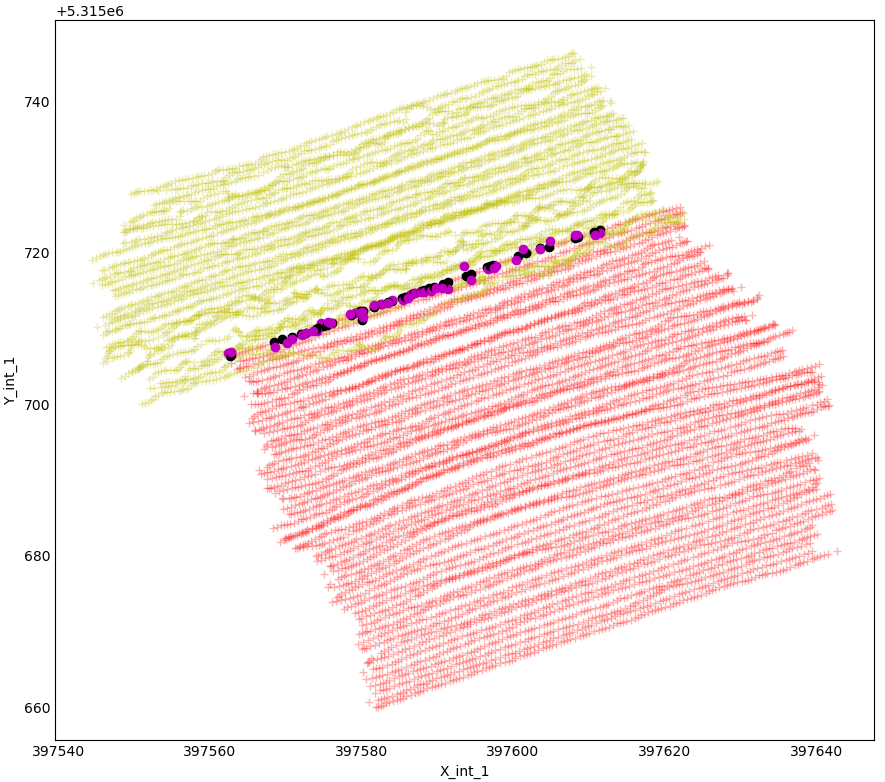
\includegraphics[width=0.8\textwidth]{Images/Frontiere_pts1-3.png}
            \caption[]%
            {{ \small Ensembles avec "superposition".}}    
        \end{subfigure}
        \hfill
        \begin{subfigure}[b]{0.418\textwidth}  
            \centering 
            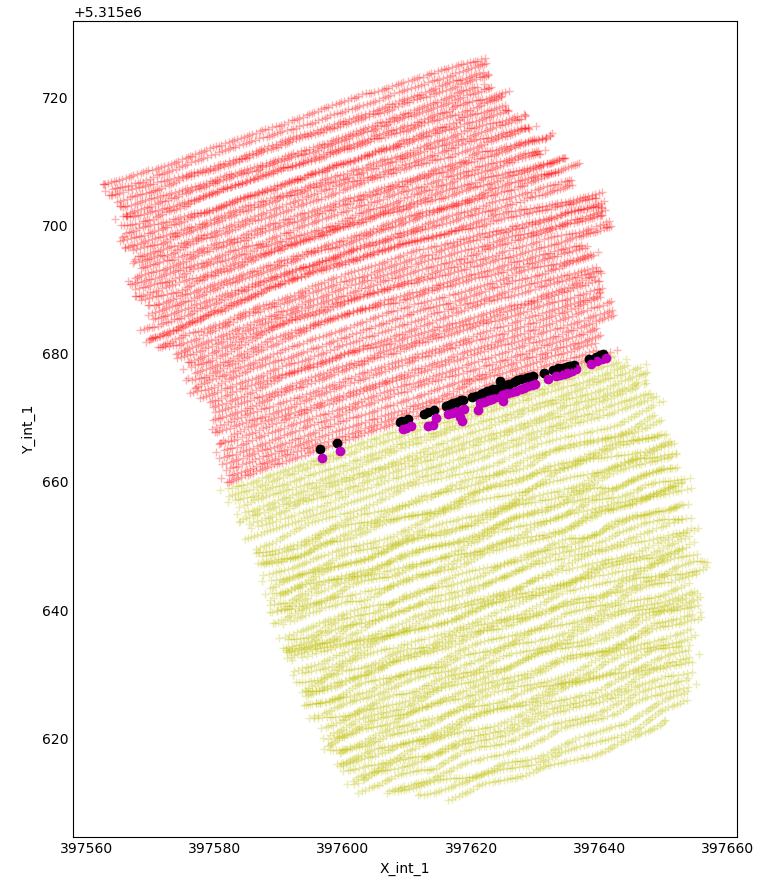
\includegraphics[width=0.8\textwidth]{Images/Frontiere_pts1-2.png}
            \caption[]%
            {{\small Ensembles frontaliers.}}    
        \end{subfigure}
        \caption{\label{fig:2_f}25 duos de points sur la frontière, détectés par l'algorithme.}
    \end{figure}
    
    À chaque itération, on avance d'un point soit sur $E_1$ soit sur $E_2$. Aucun point n'est parcouru plusieurs fois. Par conséquent, le nombre d'itération de l'algorithme est toujours égal à $|E_1| + |E_2|$. On notant $n$ le nombre total de points des deux jeux, cette méthode permet donc de trouver en $O(n)$ un minimum local du problème tout en restant plutôt facile à mettre en place \label{2_detec_front_out} (\ref{2_detec_front_in}).
    
    Il y a néanmoins plusieurs correctifs à apporter pour palier à certains problèmes. Afin 
    d'éviter les doublons lors de plusieurs itérations, on ne prendra que les points non déjà choisi par l'algorithme. De plus, un biais important peut survenir en fonction du point de départ choisi (pour un même point, on retombe toujours dans la même zone). Ces points seront donc tirés au hasard sur les deux ensembles. Enfin, deux ensembles trop éloignés ne peuvent pas partager de frontières. Il faut donc considérer une distance maximale pour considérer ou non la frontière trouvée (figure \ref{fig:2_f}).

    Si les fichiers de données contiennent des bases, c'est-à-dire des points servant uniquement à l'étalonnage, il faut les retirer au préalable pour ne pas fausser l'écart. En effet, toutes les bases d'une même prospection sont en principe faites au même endroit.
    
    On représente les points choisis en violet et noir. On constate que les distances entre les deux couleurs sont plutôt bien minimisées et se répartissent sur l'ensemble de la frontière.
    
    Selon les hypothèses du modèle, on peut s'attendre à ce que ces points soient suffisament représentatifs de la frontière pour pouvoir effectuer un ajustement efficace par la suite.

    On s'assure de ce que les ensembles non frontaliers ne soient pas détectés comme tels. Par exemple, les deux cas suivants sont exclus :

    \begin{figure}[ht!]
        \centering
        \begin{subfigure}[b]{0.475\textwidth}
            \centering
            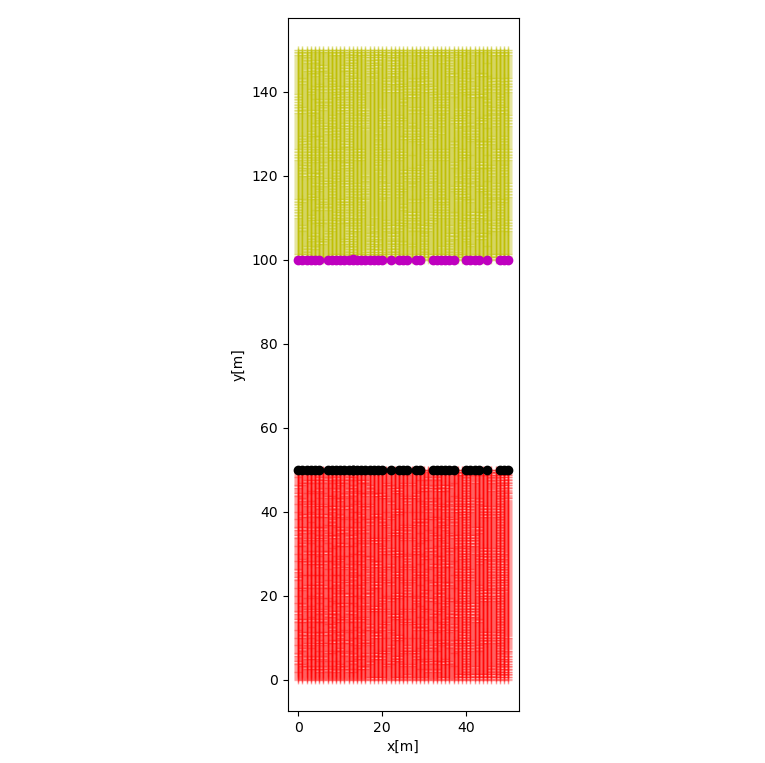
\includegraphics[width=\textwidth]{Images/Frontiere_pts_carre1-5.png}
            \caption[]%
            {{ \small Ensembles trop éloignés.}}    
        \end{subfigure}
        \hfill
        \begin{subfigure}[b]{0.475\textwidth}  
            \centering 
            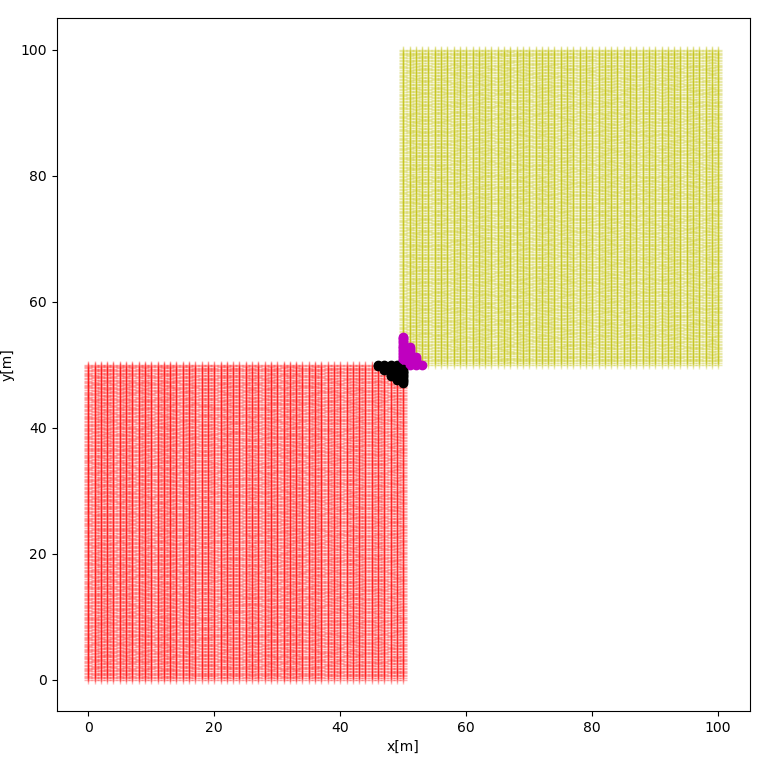
\includegraphics[width=\textwidth]{Images/Frontiere_pts_carre1-3.png}
            \caption[]%
            {{\small Ensembles en contact par un coin.}}    
        \end{subfigure}
        \caption{Cas d'exclusion de frontière.}
    \end{figure}

\newpage
\subsubsection{Ajustement des données}
    
    On approxime la déformation des données par un modèle linéaire $X = aX' + b$ avec $X'$ la donnée mesuré, $X$ la donnée réelle, $a$ le ratio des écarts types de $E_1^f$ et $E_2^f$ et $b$ la différence de moyenne entre $E_1^f$ et $E_2^f$. On applique cette transformation sur l'ensemble $E_2$.

    \begin{figure}[ht!]
        \centering
        \begin{subfigure}[b]{0.475\textwidth}
            \centering
            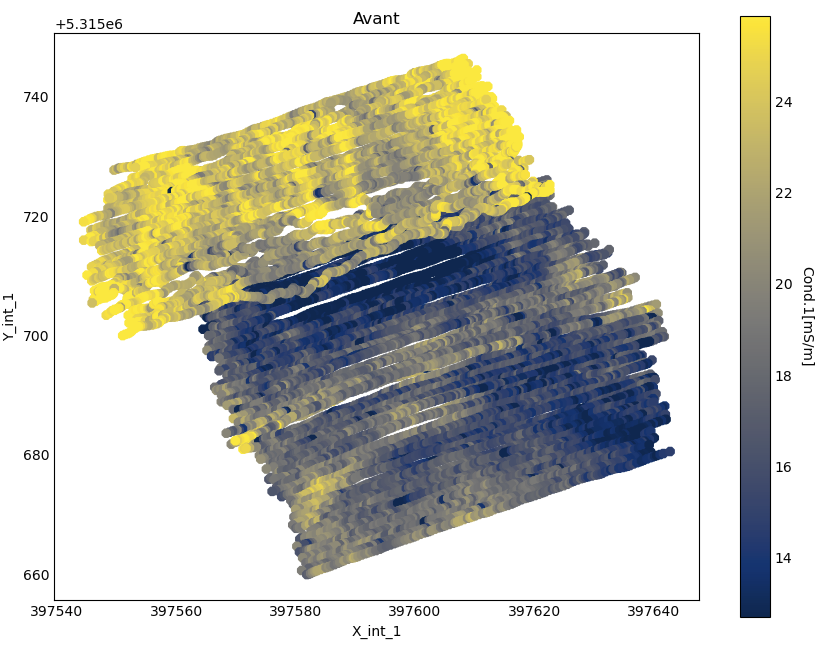
\includegraphics[width=\textwidth]{Images/Frontiere_ajust1-3_Avant.png}
            \caption[]{Avant.}
        \end{subfigure}
        \hfill
        \begin{subfigure}[b]{0.475\textwidth}  
            \centering 
            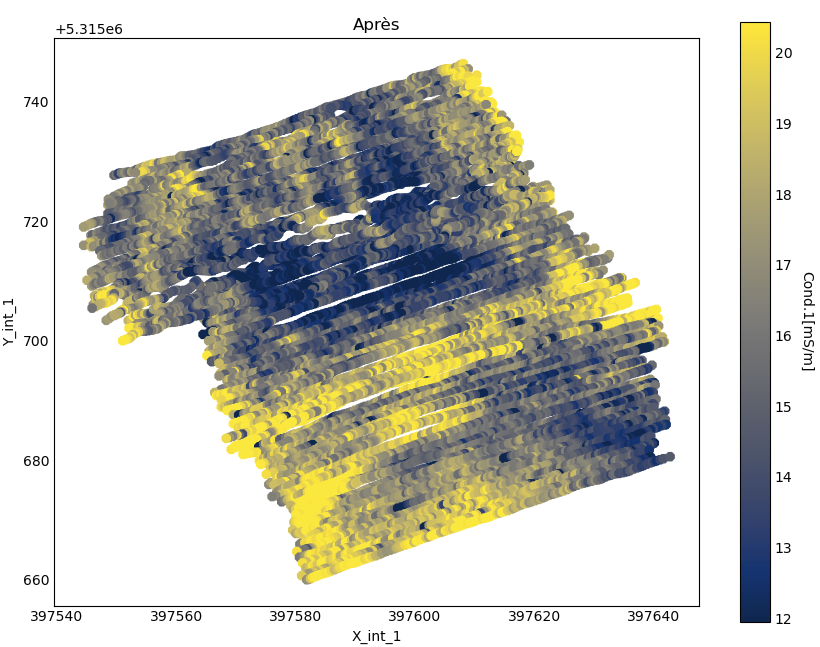
\includegraphics[width=\textwidth]{Images/Frontiere_ajust1-3_Apres.png}
            \caption[]{Après.}
        \end{subfigure}
        \caption{\label{2_avant_apres}Jeu de données avant et après ajustement.}
    \end{figure}

    Par exemple, ici (figure \ref{2_avant_apres}), j'ai volontairement bruité le second ensemble par une constante pour renforcer le décalage. On remarque que suite à la rectification, les deux ensembles de points ne sont plus discernables, ce qui souligne une meilleur cohérence des données.

    Cependant, il peut arriver que l'ajustement proposé dégrade la continuité. En effet, le choix aléatoire et non exhaustif des points couplé à l'erreur intrinsèque du modèle linéaire peut créer un "faux positif" et mal évaluer l'écart entre deux ensemble. Cela peut aussi arriver si un existe un biais fort sur la récolte, comme par exemple si l'appareil est encore en train de démarrer. Si ce cas ne fait pas majorité, on pourrait chercher à le supprimer.
    
    \label{2_detec_front_ex2_out} Pour cette raison, si il le souhaite, l'utilisateur pourra activer un mode plus manuel où il peut valider ou non chaque transformation proposée (pour chaque variable). On peut espérer obtenir un résultat final encore meilleur (\ref{2_detec_front_ex2_in}). En revanche cette étape ne concerne pas les déformations internes à un fichier. Tenter d'évaluer les frontières avant de régler les sauts internes risque de fausser les résultats.

\newpage
\subsection{Détection pseudo-profils}

    La découpage en profils est important pour permettre par la suite de corriger des déformations dû à l'appareil (voir \ref{2-etal}). Or cette information est absente du fichier de données, on doit donc la recréer. Pour cela on a besoin de procéder différemment en fonction du type de prospection réalisée.

    \begin{enumerate}
        \item[$\bullet$] Si l'appareil ne possède pas de données GPS, on est dans un cas trivial. La position (notée \texttt{"x[m]"} et \texttt{"y[m]"}) est indicative d'une cartographie en position relative (souvent par carré de prospection), où chaque profil suit l'axe $y$. Il suffit donc de commencer un nouveau profil à chaque fois que le $x$ change.
        \item[$\bullet$] Dans la majorité des cas où l'appareil utilise une antenne GPS, l'utilisateur commence par une base. Puis, il prospecte le terrain en marquant une pose entre chaque profil. Il peut de temps en temps revenir mesurer une base. Pour correctement découper la prospection en profils et bases, il faut détecter les changements brutaux de temps et surveiller si le profil trouvé est positionné au même endroit que la première base.
        \item[$\bullet$] Il peut arriver qu'une prospection utilises une antenne GPS, mais qu'elle soit réalisée sans s'arrêter. Par exemple, cela peut être le cas en mesure point par point ou sur de faibles surfaces. Dans ce cas, on ne trouvera aucun saut dans le temps. De plus, la trajectoire ne sera pas parfaitement linéaire car la jonction entre deux profils (en demi-cercle) est à prendre en compte, et on doit de toute manière pouvoir gérer des profils qui dévient de leur trajectoire.
    \end{enumerate}

    Le premier cas ne pose pas de problème particulier, et le second est déjà traité avant le stage. On va donc dans cette partie chercher une solution au troisième cas.

    En particulier on fait les tests sur les deux cas problématiques suivants :

    \begin{figure}[ht!]
        \centering
        \begin{subfigure}[b]{0.475\textwidth}
            \centering
            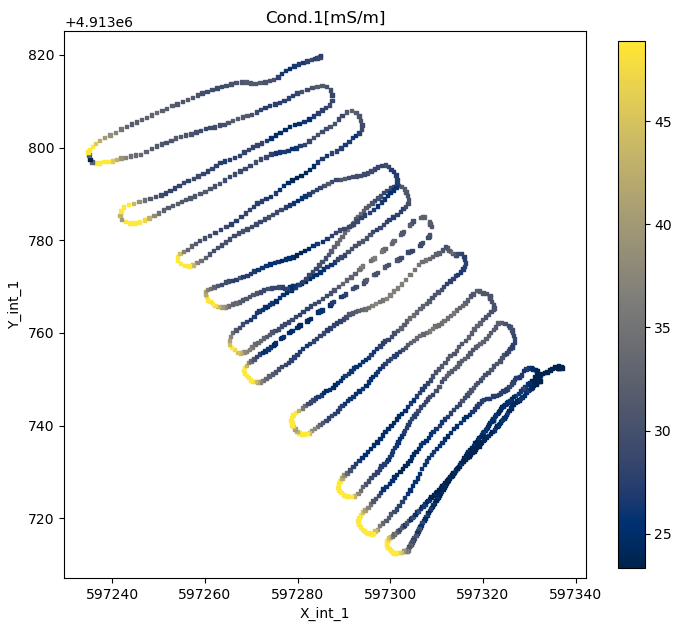
\includegraphics[width=0.925\textwidth]{Images/PseudoProf_1.png}
            \caption[]{{ \small Profils clairs avec virages.}}    
            \label{fig:2_pp_1}
        \end{subfigure}
        \hfill
        \begin{subfigure}[b]{0.475\textwidth}  
            \centering 
            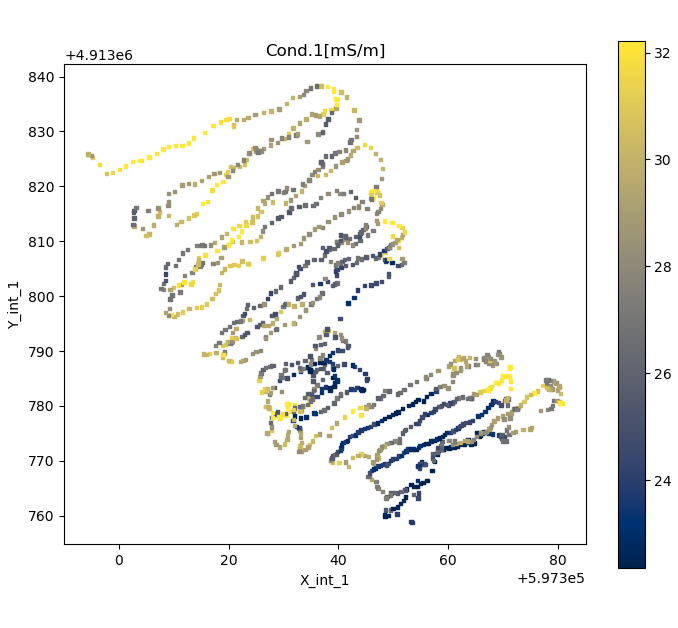
\includegraphics[width=0.925\textwidth]{Images/PseudoProf_2.png}
            \caption[]{{\small Profils chaotiques à tailles variables.}}    
        \end{subfigure}
        \caption{Différents exemples à régler.}
    \end{figure}

    Puisque la définition de profils est ambigü au vu de leur possible non linéarité, on parlera plutôt de pseudo-profils.

    \noindent\textbf{\underline{Solution envisagée}} :
    \begin{enumerate}
        \item[$\bullet$] \textbf{Points à intervalles réguliers} : Au lieu de chercher à se reporter à des pseudo-profils, on pourrait choisir de prendre un point par intervalle régulier (1 point tous les 50 par exemple) ou à proportion régulière (50 points répartis proportionnellement). Déterminer de tels points ne nécessite aucun calculs particulier, et on pourra alors choisir la médiane sur le voisionnage des points pour être représentatif de la zone choisie. Malheureusement, cette solution est inexploitable à cause de la déformation du terrain. Il n'est pas possible de faire la différence entre le terrain et le biais de l'appareil. Par exemple sur le jeu \ref{fig:2_pp_1}, la partie gauche va fausser la mesure.
    \end{enumerate}
    \textbf{\underline{Solution choisie}} : \textbf{Centres de profils} : On cherche à déduire le centre des profils sans aucune information de départ. Si on y arrive, alors on pourra associer chaque point à un centre en fonction de l'ordre de prospection et donc recréer un découpage se rapprochant d'un profil.

    \subsubsection{Régression linéaire}

    Afin d'estimer les centres des profils, on souhaite déterminer une droite passant par les centres par régression. Une fois fait, on pourra calculer la distance à la droite en tout point du jeu de données.

    La forme la plus évidente pour cela est de passer par une équation de droite de la forme $ax + by + c = 0$. Cependant, une régression classique de $y$ par rapport à $x$ ne donne pas cette information, car les coefficients $slope$ et $intercept$ trouvés correspondent à une forme $y = slope*x + intercept$, plus restrictive. Par exemple une droite d'équation $x = 5$ n'est pas représentable sous cette forme.

    Par conséquent, on utilise un raisonnement se basant sur l'ordre de prospection. On effectue une régression linéaire sur l'indice des lignes et $x$ et $y$. De cette manière, on obtient les 4 constantes répondant au système suivant :

    \begin{spacing}{1}
        \begin{equation}
            \scalebox{1.25}{$
            \begin{cases}
                x = a_xi + b_x \\
                \\
                y = a_yi + b_y
            \end{cases}
            $}
        \end{equation}
    \end{spacing}
    
    où $i$ est l'indice des lignes et $a_x$,$a_y$,$b_x$,$b_y$ les constantes des deux régressions. On cherche ensuite à retirer $i$ du calcul pour ne laisser que $x$ et $y$ en ligne de compte. Pour cela, on exprime $i$ en fonction des deux autres :

    \begin{spacing}{1}
        \begin{equation}
            \scalebox{1.25}{$
            \begin{cases}
                i = \frac{x - b_x}{a_x} \\
                \\
                i = \frac{y - b_y}{a_y}
            \end{cases}
            $}
        \end{equation}
    \end{spacing}

    La relation finale doit être une droite, donc on au moins l'un de $a_x$ et $a_y$ est non nul (sinon le résultat est un point). Le système étant symétrique, on pourra choisir la relation que l'on veut. Pour l'exemple prenons la première :

    \begin{spacing}{1}
        \begin{equation}
            \scalebox{1.25}{$y = a_y\frac{x - b_x}{a_x} + b_y$}
            \implies
            \scalebox{1.25}{$y = \frac{a_y}{a_x}x - \frac{a_y}{a_x}b_x + b_y$}
        \end{equation}
        \begin{equation}
            \implies
            \scalebox{1.25}{$a_xy - a_yx + b_xa_y - b_ya_x = 0$}
        \end{equation}
        \begin{equation}
            \implies
            \scalebox{1.25}{$\textcolor{red}{a_y(x - b_x) - a_x(y - b_y) = 0}$}
        \end{equation}
    \end{spacing}

    On obtient une équation de droite exploitable. On cherche maintenant à établir une distance point/droite. La distance effective est calculée selon \href{https://fr.wikipedia.org/wiki/Distance_d%27un_point_%C3%A0_une_droite#Dans_le_plan}{la relation suivante} :

    \begin{spacing}{1}
        \begin{equation}
            \scalebox{1.25}{$d = \frac{|a_y(x - b_x) - a_x(y - b_y)|}{\sqrt{a_x^2 + a_y^2}}$}
        \end{equation}
    \end{spacing}

    Puisqu'on cherche à comparer les distances, on peut ignorer le terme constant au dénominateur, ce qui laisse simplement à calculer la valeur absolue du terme de l'équation de droite, à savoir.

    \begin{spacing}{1}
        \begin{equation}
            \scalebox{1.25}{$\textcolor{red}{\delta = |a_y(x - b_x) - a_x(y - b_y)|}$}
        \end{equation}
    \end{spacing}

    Pour s'en assurer, on vérifie la conservation des ratios entre $d$ et $\delta$ :

    \begin{spacing}{1}
        \begin{equation}
            \scalebox{1.25}{$\frac{\delta_1}{\delta_2} = \frac{\delta_1}{\delta_2}\frac{\sqrt{a_x^2 + a_y^2}}{\sqrt{a_x^2 + a_y^2}} = \frac{\frac{\delta_1}{\sqrt{a_x^2 + a_y^2}}}{\frac{\delta_2}{\sqrt{a_x^2 + a_y^2}}} = \frac{d_1}{d_2}$}
        \end{equation}
    \end{spacing}

    Ce calcul est très rapide à effectuer.
    
    Pour déterminer quels sont les centres des profils, on choisira les minimums locaux de l'évolution des distances. En revanche, ce critère seul ne suffit pas. Les irrégularités des profils créent des minimums locaux éloignés de la courbe, en témoigne leur présence en dehors des creux (croix rouges, figure \ref{pp_1}).

    \begin{figure}[ht!]
        \centering
        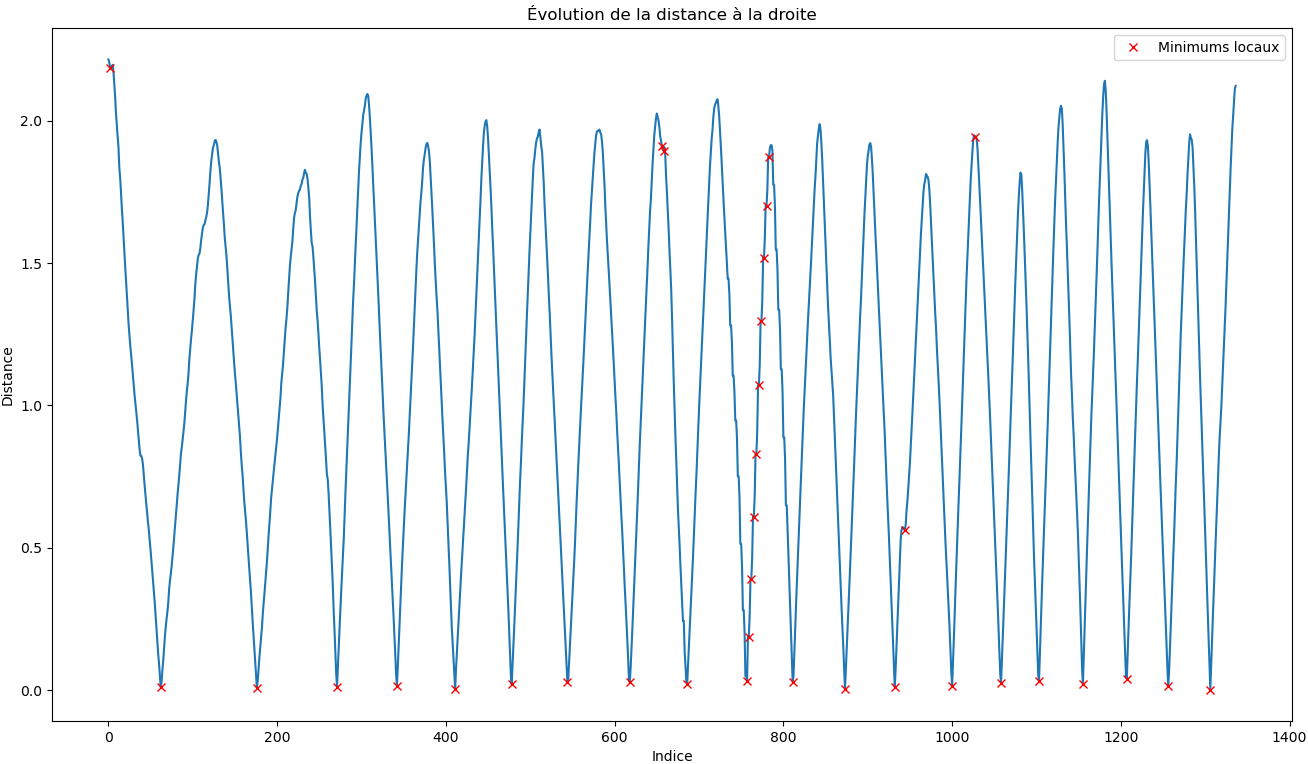
\includegraphics[width=0.98\textwidth]{Images/PseudoProf_dist_1.png}  
        \caption{\label{pp_1} Évolution de la distance à la droite par rapport à l'indice, jeu 1.}
    \end{figure}

    On doit donc éliminer ensuite ces points. On prend comme valeur de seuil \texttt{tn\_c = 20} fois la moyenne des \texttt{tn = 10} points à distance minimale, en supposant qu'une prospection devrait comprendre au moins 10 profils (et donc au moins 10 points très proches de la droite).

    \vskip 15pt
    
    Malgré cela, il existe deux derniers cas gênant. En premier lieu, celui de détecter deux fois le même profil (croix rouges, figure \ref{pp_2}).

    Si deux points sont espacés de moins de \texttt{min\_conseq = 8} en indice, le plus éloigné sera retiré. On considère qu'un profil devrait mesurer au moins 8 points et que si deux points du même profil sont plus espacés, alors au moins l'un d'entre eux sera suffisament excentré pour être éliminé suite au premier filtre. Si un profil revient sur ses pas après plus de 8 points, la procédure va le considérer comme deux profils distincts.

    En second lieu, si certains profils sont trop éloignés de la droite des centres, il est possible qu'il ne se touchent pas. Dans ce cas, on mesurera des profils bien trop grand qui en sont en réalité plusieurs. Par conséquent, si deux centres sont plus éloignés que le double de la médiane des écarts, on coupera la zone entre les deux en insérant des centre arbitraires.

    Enfin, pour chaque point du jeu, on lui associe le centre trouvé le plus proche. L'indice de ce centre dans la liste des centres permettra de numéroter le profil.

    \begin{figure}[ht!]
        \centering
        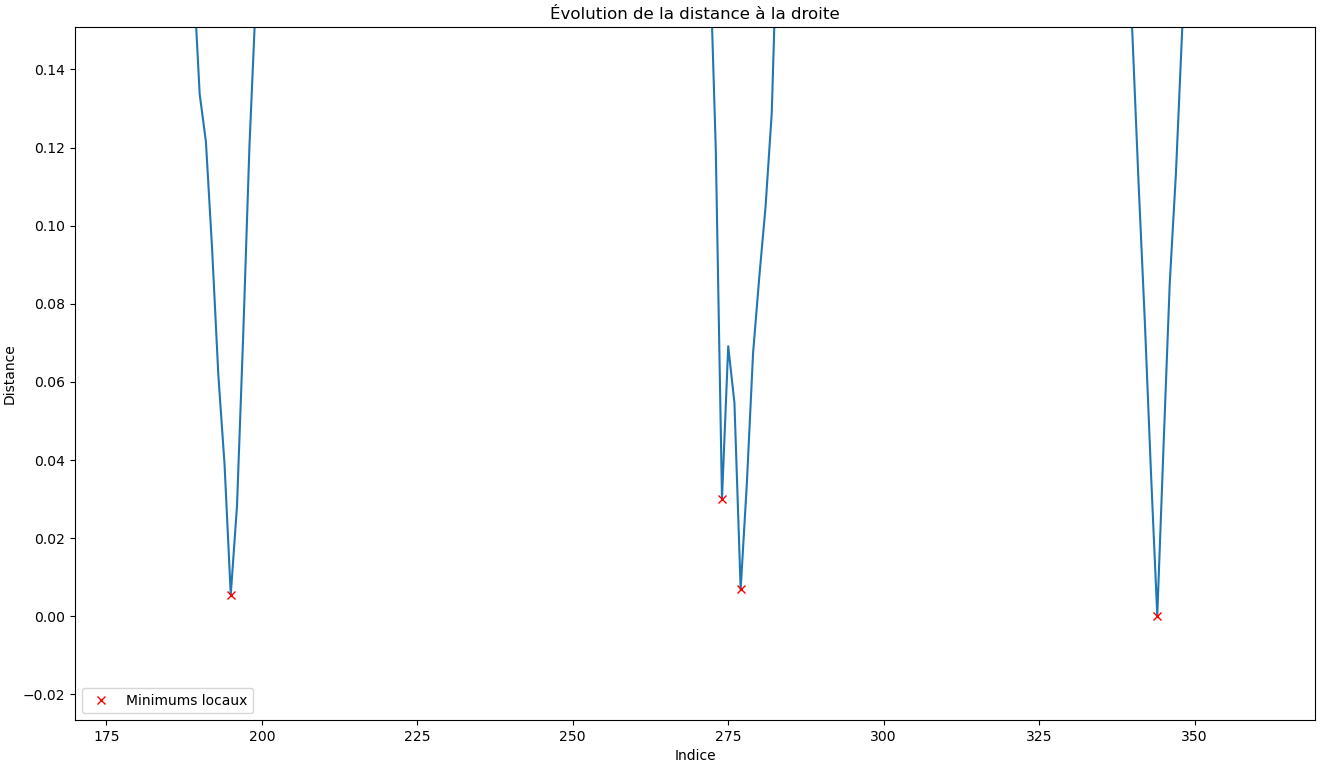
\includegraphics[width=0.98\textwidth]{Images/PseudoProf_dist_2.png}  
        \caption{\label{pp_2} Extrait de l'évolution de la distance à la droite par rapport à l'indice, jeu 2.}
    \end{figure}
    \newpage
    Résultat :
    \begin{figure}[ht!]
        \centering
        \begin{subfigure}[b]{0.90\textwidth}
            \centering
            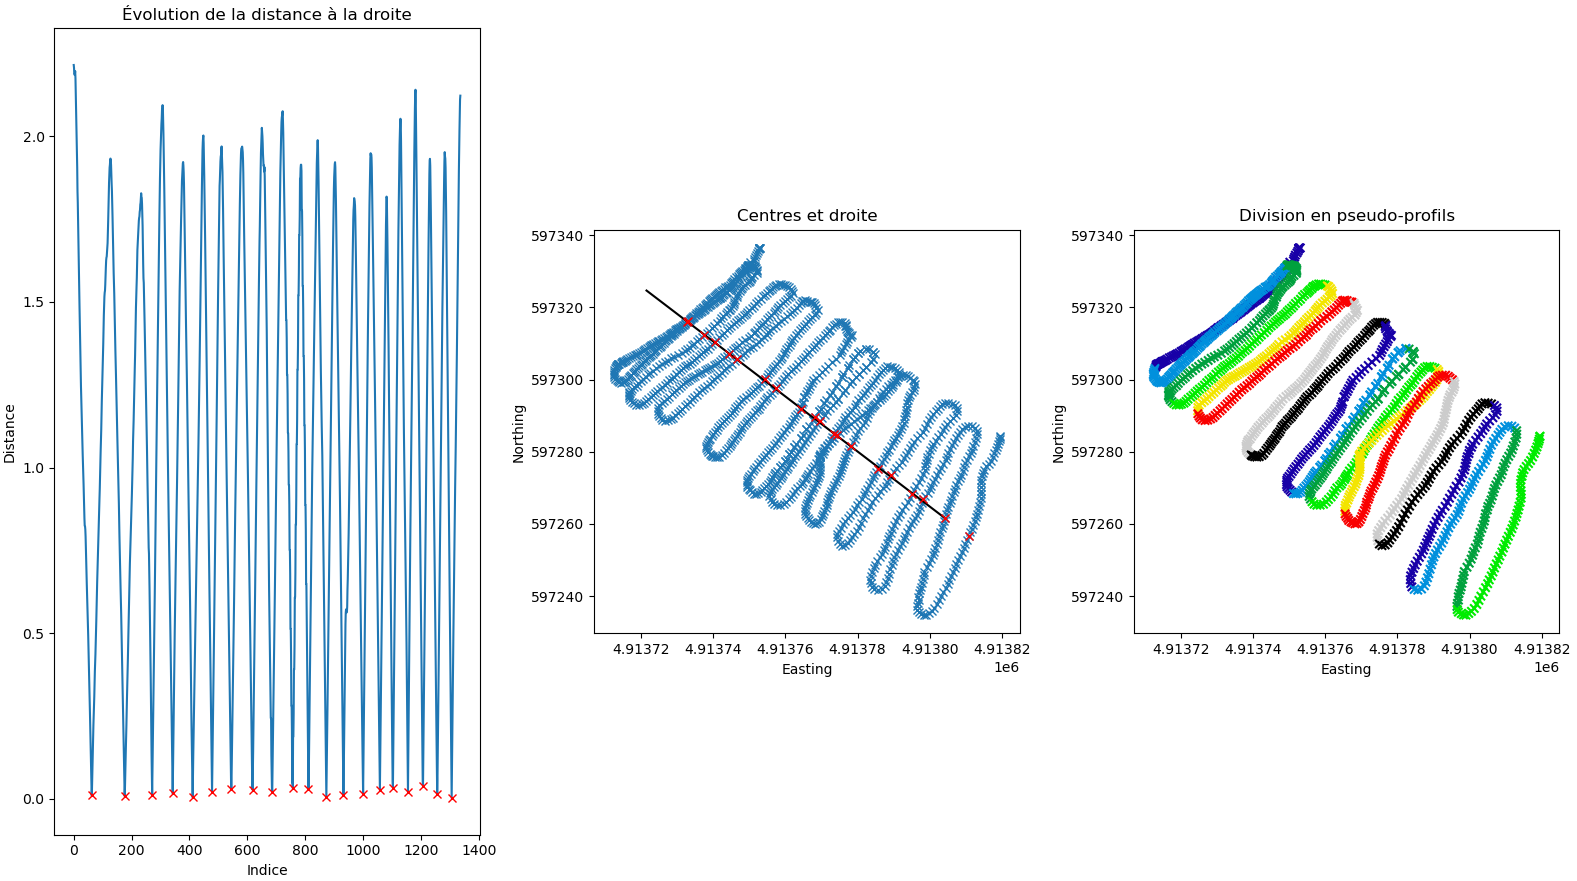
\includegraphics[width=\textwidth]{Images/PseudoProf_full_1.png}
            \caption[]%
            {{ \small Jeu 1 (facile).}}    
        \end{subfigure}
        \centering
        \begin{subfigure}[b]{0.90\textwidth}  
            \centering 
            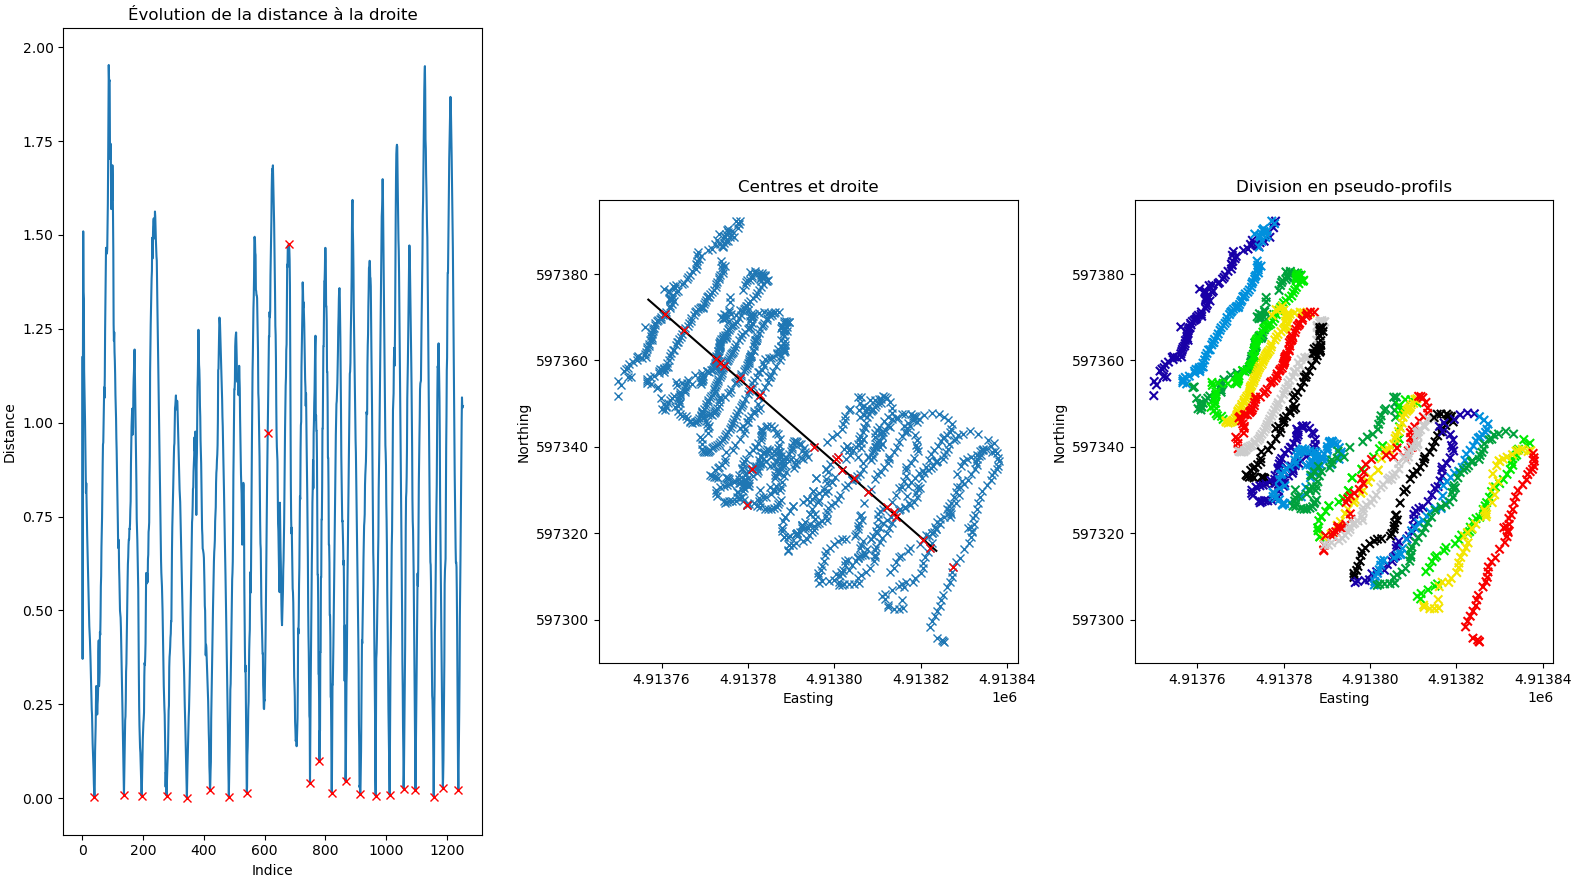
\includegraphics[width=\textwidth]{Images/PseudoProf_full_2.png}
            \caption[]%
            {{\small Jeu 2 (difficile).}}   
            \label{fig:2_pp_2}
        \end{subfigure}
        \caption{Découpage en pseudo-profils proposé.}
    \end{figure}

    \newpage
    \subsubsection{Découpage en segments}

    On remarque sur la figure \ref{fig:2_pp_2} que le découpage du bloc en bas à gauche n'est pas optimal, et qu'on aimerait que la droite coupe ses profils. Dans ce cas, il est intéressant de considérer une succession connexe de segments pour le calcul de la distance. De cette manière on peut s'assurer que tous les profils sont traversés.

    Les $n$ segments seront construits avec les coordonnées de $n+1$ points spécifiés par l'utilisateur. On s'assure donc d'avoir en entrée au moins deux points.

    Afin de calculer la distance entre un point $p$ et un segment $[A,B]$, on effectue un test sur les angles $\widehat{pAB}$ et $\widehat{pBA}$. On suit la procédure suivante :

    \begin{spacing}{1}
        \begin{equation}
            \scalebox{1.25}{$
            \begin{cases}
                \widehat{pAB} > 90° \implies d = ||\overrightarrow{pA}|| \\
                \widehat{pBA} > 90° \implies d = ||\overrightarrow{pB}|| \\
                sinon \implies d = \frac{||\overrightarrow{AB}\land\overrightarrow{Ap}||}{||\overrightarrow{AB}||}
            \end{cases}
            $}
        \end{equation}
    \end{spacing}

    On réalise le calcul pour chaque segment et on garde le minimum. On a donc un nouveau calcul de distance (cette fois-ci exact).

    Puisque les segments en entrée sont censés traverser tous les profils (sinon le choix n'a pas d'intérêt), on ignore la procédure de rajout de centres sur grands blocs.

    \begin{figure}[ht!]
        \centering
        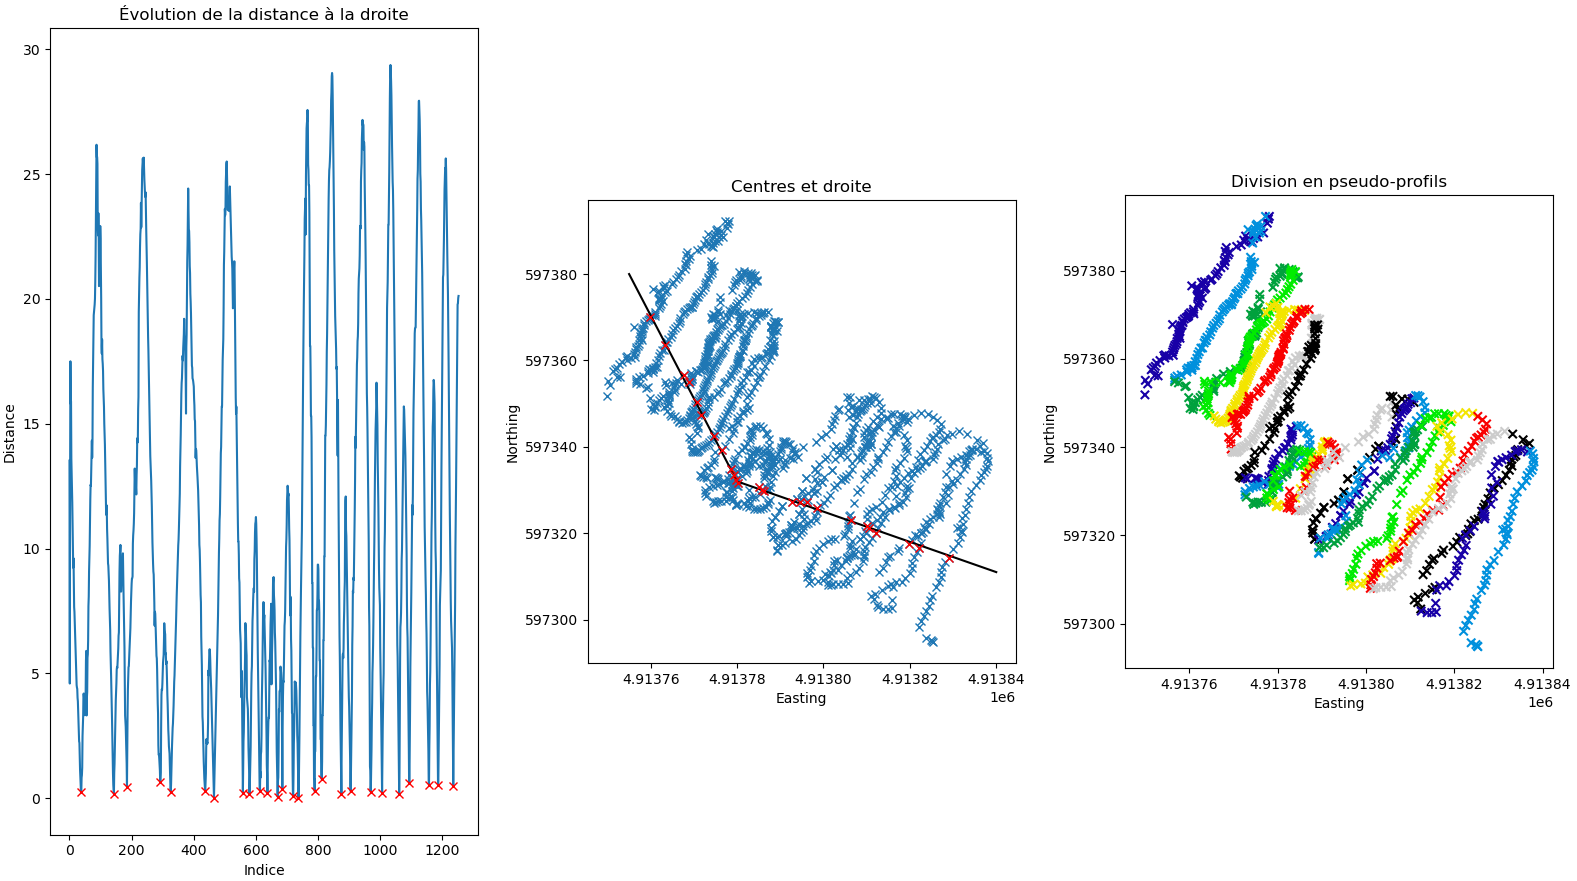
\includegraphics[width=\textwidth]{Images/PseudoProf_full_2_seg.png}  
        \caption{Découpage en pseudo-profils proposé, jeu 2.}
        \label{fig:2_pp_2_seg}
    \end{figure}

    \subsubsection{Remarques sur la procédure}

    Cet algorithme utilise des valeurs arbitraires pour retirer certains minimums locaux de la liste des centres. Les valeurs associées aux paramètres \texttt{tn}, \texttt{tn\_n} et \texttt{min\_conseq} ne peuvent pas couvrir tous les cas. Si le résultat est imparfait, on pourra les faire varier. Par exemple, si trop de centres sont retirés, il faut augmenter \texttt{tn} et/ou \texttt{tn\_n}.

    Sur la figure \ref{fig:2_pp_2_seg}, certains profils ne sont pas coupés en leur centre. Cependant, on associe à chaque point le centre trouvé \textit{le plus proche} dans le sens des indices lors de la numérotation des profils. Si un profil est coupé par le côté, le précédent et le suivant le sont aussi (selon toute probabilité). Or puisque les profils alternent de sens, le découpage reste tout aussi correcte.

    \begin{figure}[ht!]
        \centering
        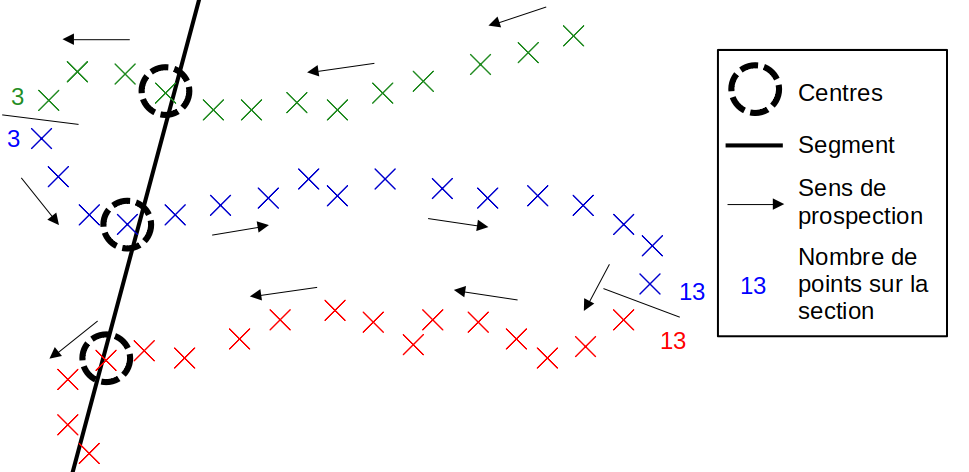
\includegraphics[width=\textwidth]{Images/PseudoProf_sch.png}  
        \caption{Stabilité de la procédure.}
    \end{figure}

    Lors de la construction de la droite ou des segments, il faut éviter de couper parallèlement à une partie d'un profil, au risque de créer pleins de centres. Dans ce cas, il est préférable de simplement changer la position des points des segments.

    Si la prospection superpose plusieurs profils dans des directions différentes, on aura du mal à les distinguer avec cette méthode. On pourra tout de même tenter de couper chaque profile une fois, mais si la trajectoire du segment ne coupe pas les profils de manière perpendiculaire, la sécurité présentée dans la figure précédente n'est plus vraie. Dans ce cas les côtés des profils ne seront pas toujours correctement associés à leur profil.
    
\newpage  
\subsection{Étalonnage des profils}\label{2-etal}
\subsubsection{Problématique et méthode utilisée pour l'étalonnage par base}

    \label{2_evol_base} Dans une partie précédente, nous avons tenté de corriger les erreurs entre différentes parcelles en se basant uniquement sur la frontière. Cela permet de répondre au problème de discontinuité, mais ne peut traiter les décalages survenant pendant la prospection d'une même parcelle , typiquement à cause de la dérive de instrumentent de mesure (figure \ref{fig:2_ep_vt}). Pour cela, on réalise des bases à des points fixes de l'espace qui serviront à uniformiser les données. Puisque qu'un même point doit donner la même valeur, on peut alors mesurer le décalage de l'appareil, à condition de revenir plusieurs fois dessus. Il s'agit d'une stratégie assez proche de celle de la frontière, mais au milieu d'une même prospection.

    Une base est constitué de plusieurs points, certains pris au sol (comme pour la prospection) ou en l'air (pour évaluer l'offset de l'appareil). On va d'abord s'intéresser uniquement aux mesures en l'air. Tout comme les profils, une série de point en base fait partie d'une même base. Pour obtenir une valeur significative, on prendra la médiane de chaque base en compte. En parallèle, on va également calculer la médiane de chaque profil pour chaque variable observée.

    On rappelle les hypothèses du modèle :
    \begin{enumerate}
        \item[\textbf{(1)}] Plusieurs mesures de base, si situées au même endroit, doivent donner les mêmes résultat. Si ce n'est pas le cas, on considère que la différence trouvée doit être corrigée car elle vient de l'appareil.
        \item[\textbf{(2)}] Les profils et les bases au sein d'une même prospection sont établis à intervalle régulier.
        \item[\textbf{(3)}] La médiane d'un profil ou d'une base est suffisament repésentative pour pouvoir établir une évolution temporelle.
        \item[\textbf{(4)}] Un décalage survenant entre deux bases évolue de manière linéaire.
    \end{enumerate}

    \begin{figure}[ht!]
        \centering
        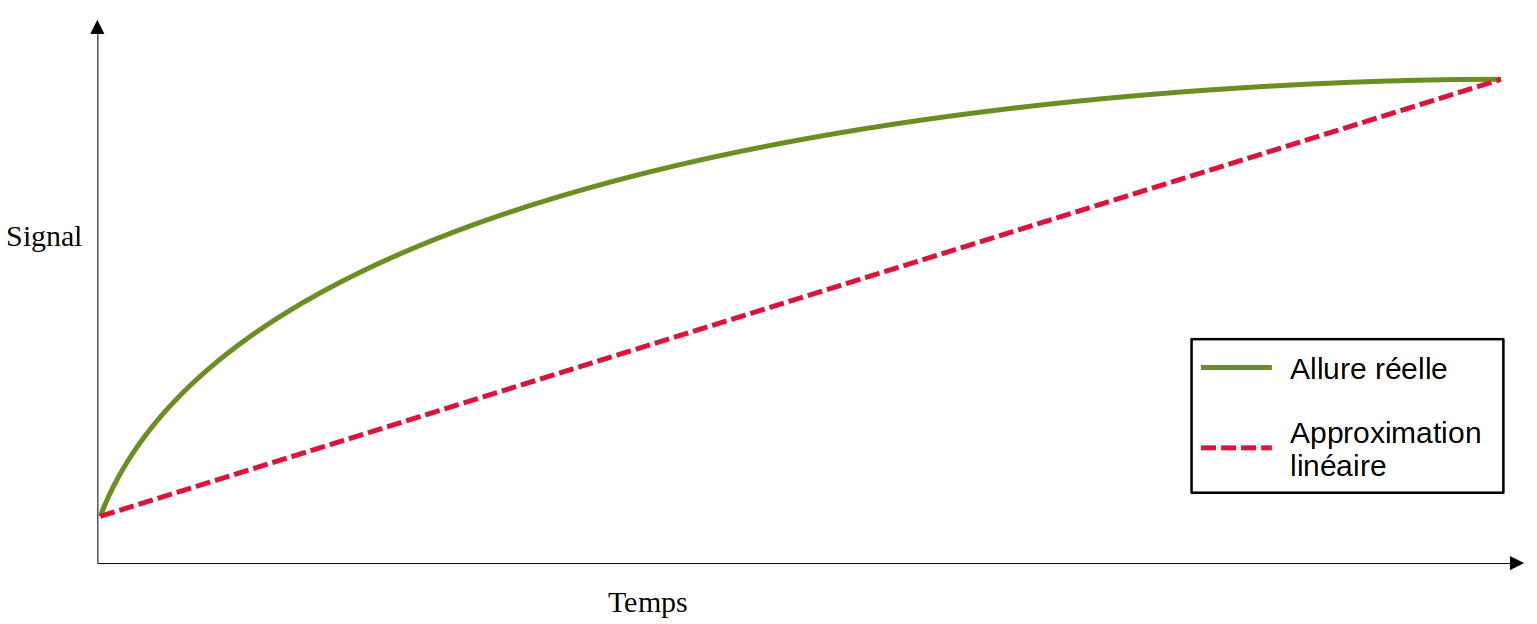
\includegraphics[width=\textwidth]{Images/Base_Vrai_Evol.png}  
        \caption{Allure de la variation théorique de la dérive de l'appareil au démarrage.}
        \label{fig:2_ep_vt}
    \end{figure}

    En réalité, le plus grand décalage est dû à un redémarrage de l'appareil. Dans ce cas, il faut attendre plusieurs minutes avant qu'il se stabilise, en suivant un évolution quadratique (figure \ref{fig:2_ep_vt}). On le remarque facilement sur l'\textit{inphase} du jeu à parcelles carrées (\ref{2_detec_front_ex2_in}). L'hypothèse \textbf{(4)} est donc imparfaite, mais plus simple à mettre en œuvre.

    Avec les hypothèse \textbf{(2)} et \textbf{(3)}, on va considérer que le numéro de chaque profil/base peut servir de marqueur temporel ; on peut donc tracer l'évolution des médianes. Pour faciliter la lecture, on prend une échelle de proportionalité car on ne s'intéresse qu'au rapport entre les médianes et non à leur valeur en brut.

\subsubsection{Ajustement des données par base}

    Dans la plupart des cas, on va préférer corriger le décalage en faisant la différence entre la base n et n+1. Ce choix est souvent plus proche du décalage du zéro de l'appareil. De cette manière, on ne modifie pas l'écart type du jeu.

    \begin{figure}[ht!]
        \centering
        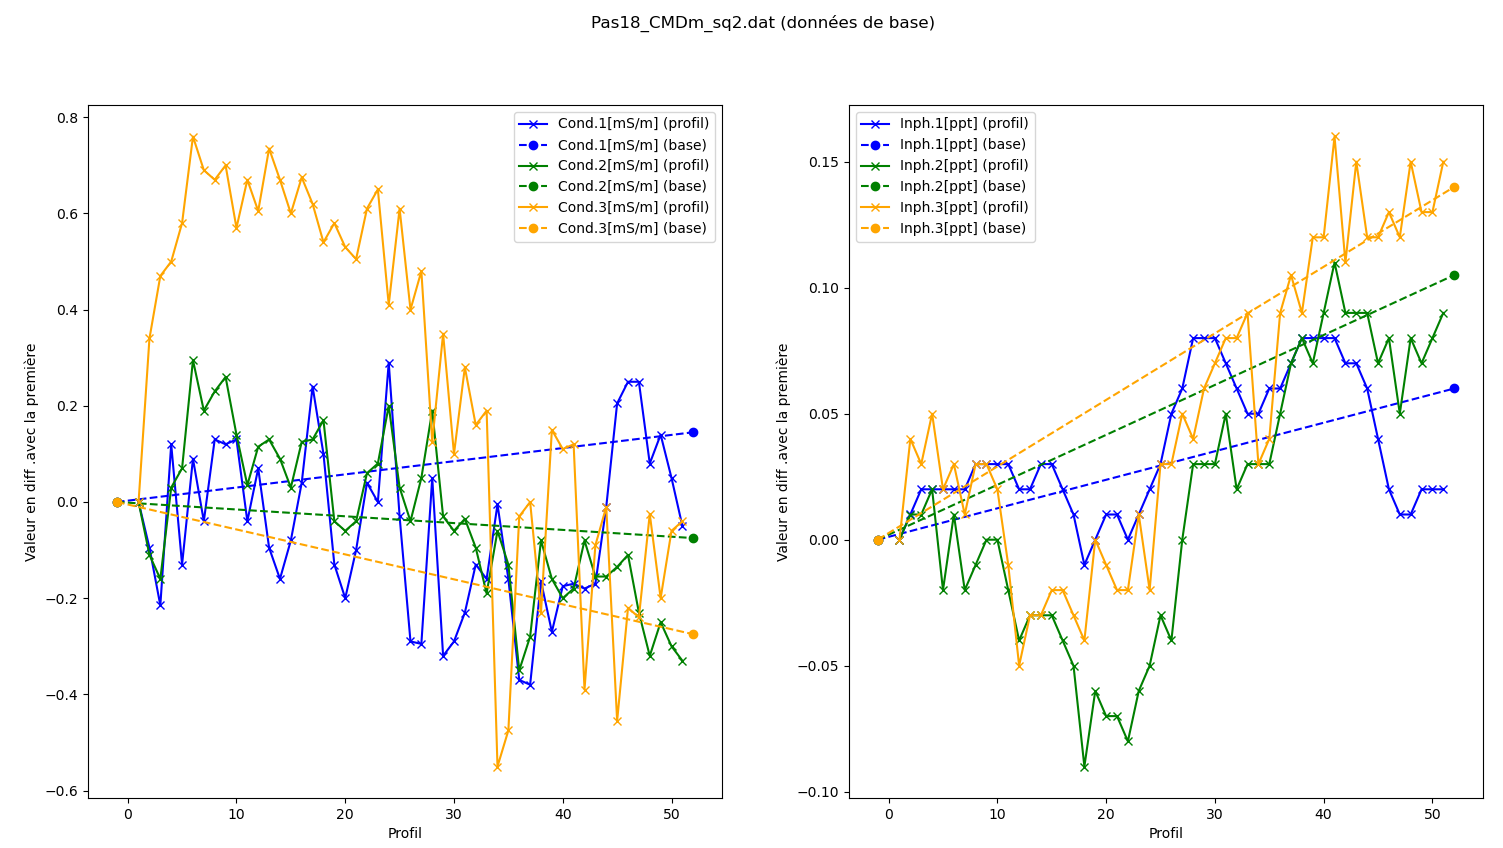
\includegraphics[width=\textwidth]{Images/Base_diff_Avant_sq2.png}  
        \caption{Médiane des bases et profils en fonction de leur ordre chronologique.}
    \end{figure}

    En prenant un jeu avec seulement une base au début et à la fin, on se rend compte que l'évolution globale (décroissante pour \texttt{Cond.}, croissante pour \texttt{Inph.}) semble être suivie à la fois par les profils et par les bases. Selon l'hypothèse \textbf{(1)}, la différence de base témoigne d'un décalage de l'appareil, décalage intervenant donc également sur les profils. On peut donc estimer qu'au moins une partie de cette évolution provient d'une erreur matérielle, celle qu'on cherche à compenser.

    Pour cela on va rabattre la valeur de la base n+1 (à droite) sur celle de la base n (à gauche, en entraînant les profils situés entre de manière linéaire.

    \newpage
    \begin{figure}[ht!]
        \centering
        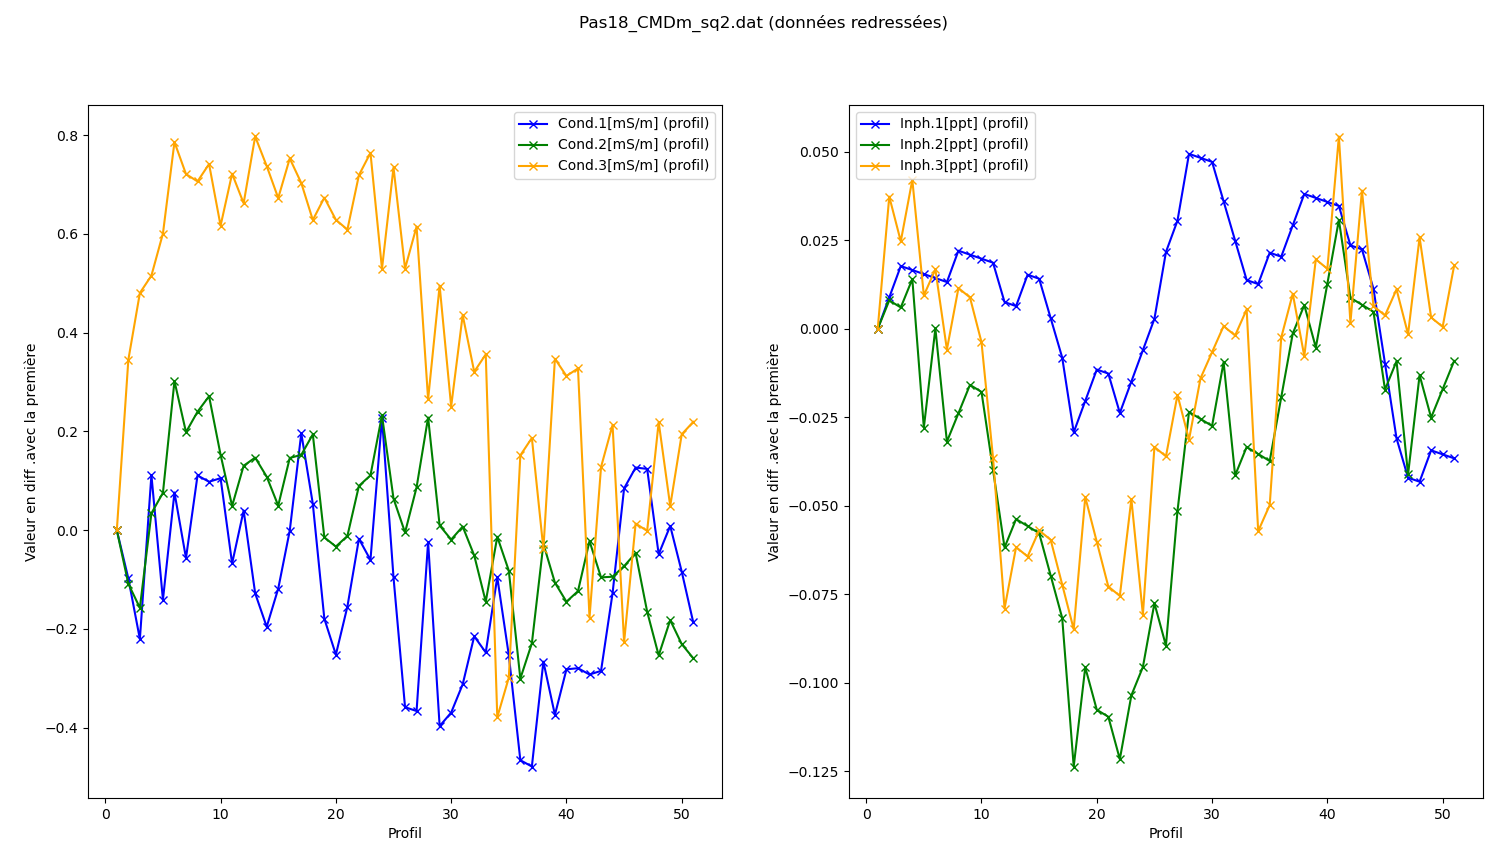
\includegraphics[width=\textwidth]{Images/Base_diff_Apres_sq2.png}  
        \caption{Médiane des profils après ajustement.}
        \label{fig:2_evol_base_im}
    \end{figure}

    Suite à cette opération (figure \ref{fig:2_evol_base_im}), on remarque que la tendance en \texttt{Cond.} est conservée, quoiqu'atténuée. Il est donc fort probable que cela viennent du terrain et soit représentatif du secteur. En revanche, \texttt{Inph.} suit désormais une évolution en N inversé, et reste plutôt stable aux extrémités. En s'en fiant aux bases, la tendance croissante était une déformation des mesures.

    En suivant la même méthode, on peut extrapoler cet ajustement avec des jeux possédant des bases au milieu de la prospection.

\subsubsection{Ajustement manuel}

    Il existe des déformations qui sont visuellement frappantes mais qui ne peuvent pas être traitées par les bases. Par exemple si aucune base n'est prise au milieu de la prospection, il est impossible de détecter le démarrage de l'appareil de cette façon. De plus on doit éviter de chercher à corriger ces déformations automatiquement, car un changement brutal dans les données n'est pas toujours dû à une erreur de l'appareil.

    \label{2_aj_man_out} Pour cela, on peut se servir du graphe des médianes. Si l'utilisateur sait qu'une déformation a eu lieue, il pourra repérer les numéros des profils concernés (en rouge) (\ref{2_aj_man_in}). On appliquera la méthode d'ajustement en prenant les profils précédents et suivant comme "base" (en bleu) pour obtenir les points interpolés (en vert).

    \label{2_aj_man_ex_out} Un exemple d'utilisation est montré en annexe (\ref{2_aj_man_ex_in}).

    Les deux méthodes (base et manuel) sont complémentaires et utilisent beaucoup de calculs en commun, mais elles ont un but différent. Pour cette raison, on laisse la possibilité de n'en appliquer qu'une des deux si on a un but plus spécifique.

\newpage
\subsection{Affichage en grille}\label{2-3}

    Jusqu'à ici, on s'est intéressé à l'affichage du nuage de point que représente les données, brut ou interpolées. Cependant, pour faciliter la visualisation de la zone, on désire s'affranchir des points et se concentrer sur un découpage en grille. Chaque case de cette grille représente un intervalle de position, et sa couleur doit être représentative des points se trouvant à l'intérieur.

    On se place dans l'ensemble des contraintes suivantes :
    \begin{enumerate}
        \item[\textbf{(1)}] La méthode doit tenir compte de tous les points de l'ensemble, ou au minimum de la répartition globale du nuage de points.
        \item[\textbf{(2)}] La valeur de chaque case doit être cohérente avec celles de ses points, et non simplement un indice de variation quelconque. Par exemple, égale à la moyenne des mesures à l'intérieur.
        \item[\textbf{(3)}] Les cases en périphérie ne contenant aucun point ne doivent pas être colorées. On évitera alors d'évaluer des territoires hors de la prospection.
        \item[\textbf{(4)}] Le temps de calcul (et donc la complexité) doit être suffisament petit pour être applicable à tout jeu de données, sans craindre de crash ou de bloquer pendant des heures.
    \end{enumerate}

\subsubsection{Découpage de la grille}

    Afin de préparer la grille d'interpolation, on définit une fonction effectuant les tâches suivantes :

    \begin{enumerate}
        \item[$\bullet$] Attribuer une valeur à chaque case en fonction des points s'y trouvant. Si la case est vide, on lui attribue la valeur spécifique $NaN$. Sinon, on indique la présence d'un point par un $0$.
        \item[$\bullet$] On ajuste le résultat trouvé en fonction des cases avoisinantes. Pour cela, on se sert d'un rayon \texttt{radius} où chaque case à l'intérieur du cercle est pondérée par un coefficient dérivé de sa distance au centre. On introduit un seuil \texttt{seuil}, servant à définir si une case précédemment vide doit être ajoutée quand même ; sinon on la laisse vide.
    \end{enumerate}

    Cette procédure permet de déterminer quelles sont les cases à exclure de l'interpolation, et donc répondre à l'exigeance \textbf{(3)}. Sa complexité est en $O(n)$ sur les données, $O(n^{2})$ sur la précision de la grille, $O(n^{2})$ sur le rayon (ce qui est optimal au vu des conditions). Le temps de calcul est raisonnable dans la majorité des cas, en général moins de dix secondes (exigeance \textbf{(4)}).

    La répartition des coefficients dépend d'une fonction polynomiale, où le paramètre \texttt{seuil} détermine la vitesse de décroissance (le degré du terme).

    Ainsi, plus le \texttt{seuil} est grand, plus on donne d'importance aux points très proche. Si \texttt{seuil} $= 0$ par exemple, on obtient une grille à coefficients constants. Il est aussi possible de considérer des \texttt{seuil}s négatifs, dans ce cas on prendra le cas \texttt{seuil} $= 0$ multiplié par $1 -$ \texttt{seuil} (pour ne pas créer d'incohérences). En l'occurence, on préférera des \texttt{seuil}s faibles (càd proches de 0) pour boucher les trous, car les cases à l'intérieur sont souvent à proximité de beaucoup de cases sans être nécessairement à 1 de distance. Cependant, si le jeu ne crée pas de trous, un fort \texttt{seuil} permet de découper plus violamment la frontière.

    \begin{figure}[ht!]
        \centering
        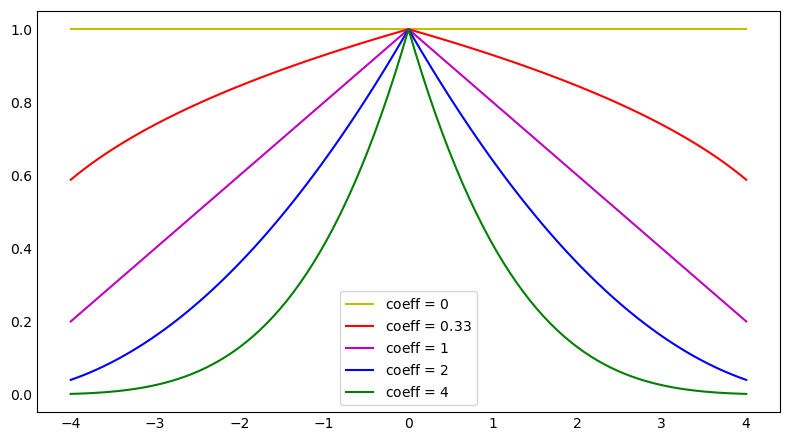
\includegraphics[width=0.8\textwidth]{Images/Grid_FirstAlg_CoeffCurve.png}
        \caption{Exemples de répartition des coefficients en fonction de la distance au centre.}
    \end{figure}
    
    \label{2_grid_firstalg_coeff_out} On peut ensuite appliquer cette loi 1D sur une grille 2D (\ref{2_grid_firstalg_coeff_in}).

\subsubsection{Heatmap}

    Afin de faciliter le choix du \texttt{seuil}, on propose de passer par une heatmap de densité de case. On affiche deux représentations (figure \ref{fig:2_heatmap}):

    \begin{enumerate}
        \item[$\bullet$] À gauche, la heatmap attribuant un score de densité à chaque case.
        \item[$\bullet$] À droite, le découpage induit, où on ne prend que les cases avec 1 de score ou plus. On représente également les points de l'ensemble initial pour pouvoir juger de la pertinence du découpage.
    \end{enumerate}

    \begin{figure}[ht!]
        \centering
        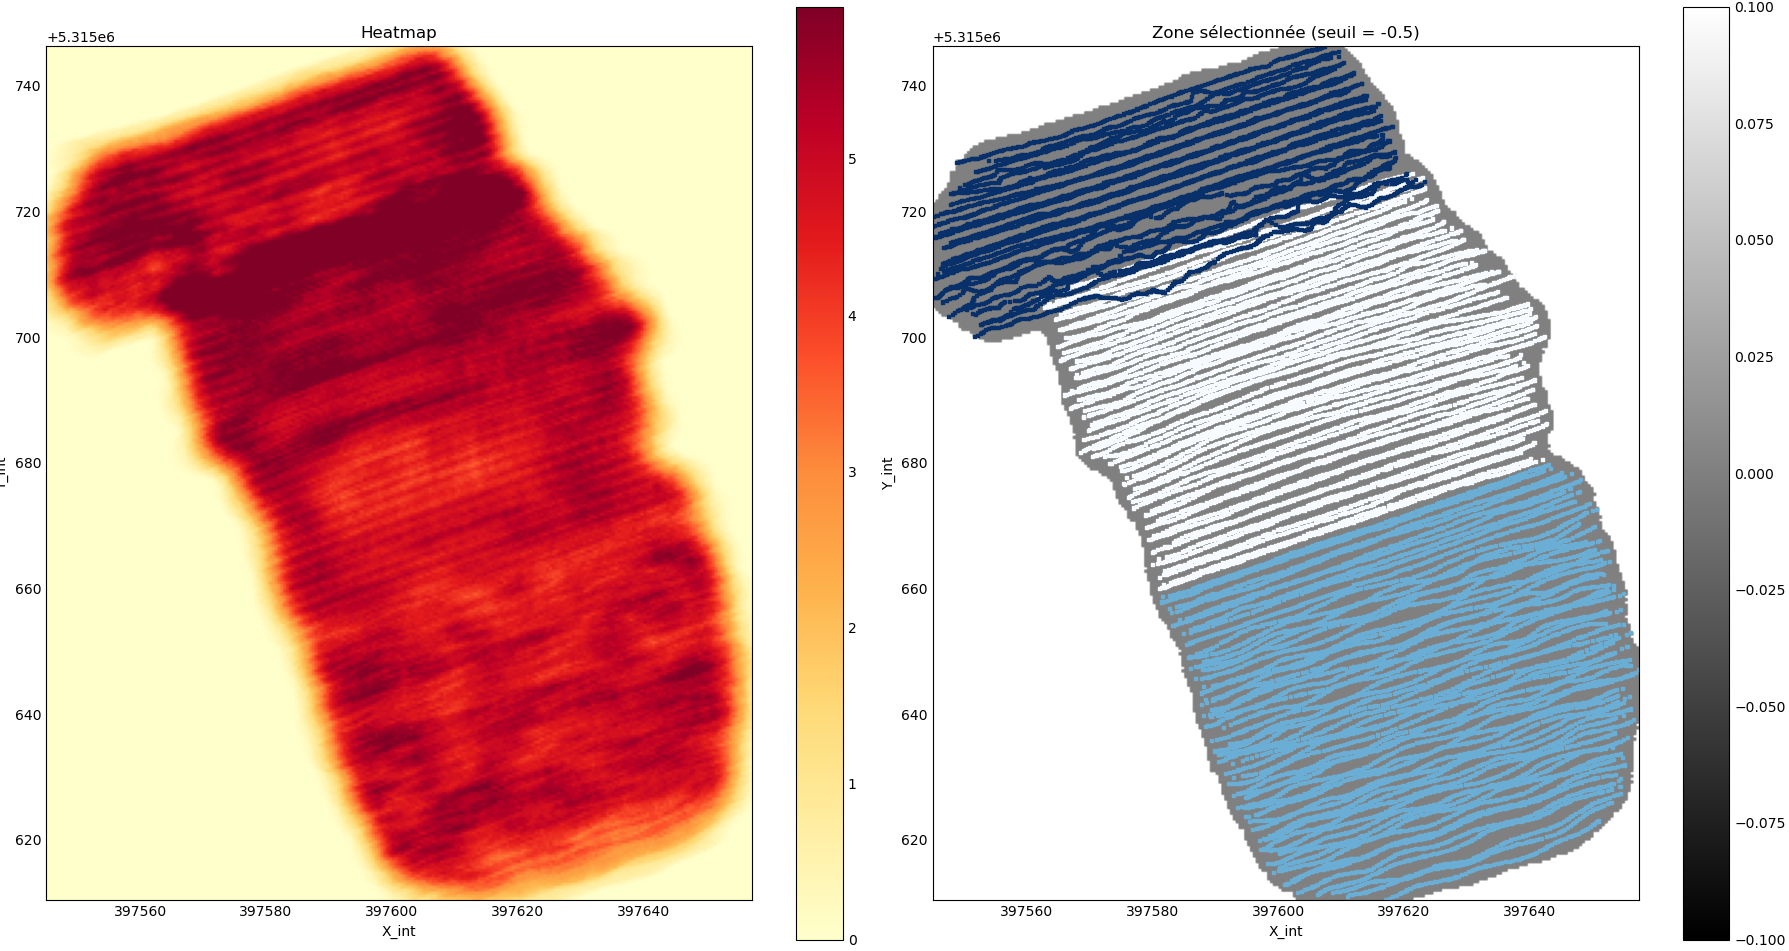
\includegraphics[width=0.8\textwidth]{Images/Grid_Heatmap_p300.png}
        \caption{\label{fig:2_heatmap}Heatmap et découpage, [\texttt{prec} = 300].}
    \end{figure}
    
    En faisant varier le \texttt{seuil}, on peut expérimenter plusieurs découpages, jusqu'à trouver celui qui correspond le mieux au jeu.

    Un fois fini, on pourra lancer une interpolation/krigeage avec le \texttt{seuil} trouvé.

    Il est important de noter que si l'on souhaite réaliser l'interpolation sur plusieurs voies d'une même prospection, on aura des coordonnées différentes. Cependant, la variation est en principe suffisament petite pour ne pas faire différer le découpage de manière significative. On peut alors se contenter d'afficher la heatmap pour le premier couple de position uniquement.

\newpage
\subsubsection{Interpolation classique}

    La solution la plus simple pour mettre en grille des données est de passer par un algorithme d'interpolation, comme fourni par la bibliothèque \href{https://docs.scipy.org/doc/scipy/reference/generated/scipy.interpolate.griddata.html}{scipy}. La fonction \texttt{griddata} propose trois types d'interpolateur : \texttt{nearest} (neighbor), \texttt{linear} et \texttt{cubic}. Leur utilisation est très rapide.

    \begin{figure}[ht!]
        \centering
        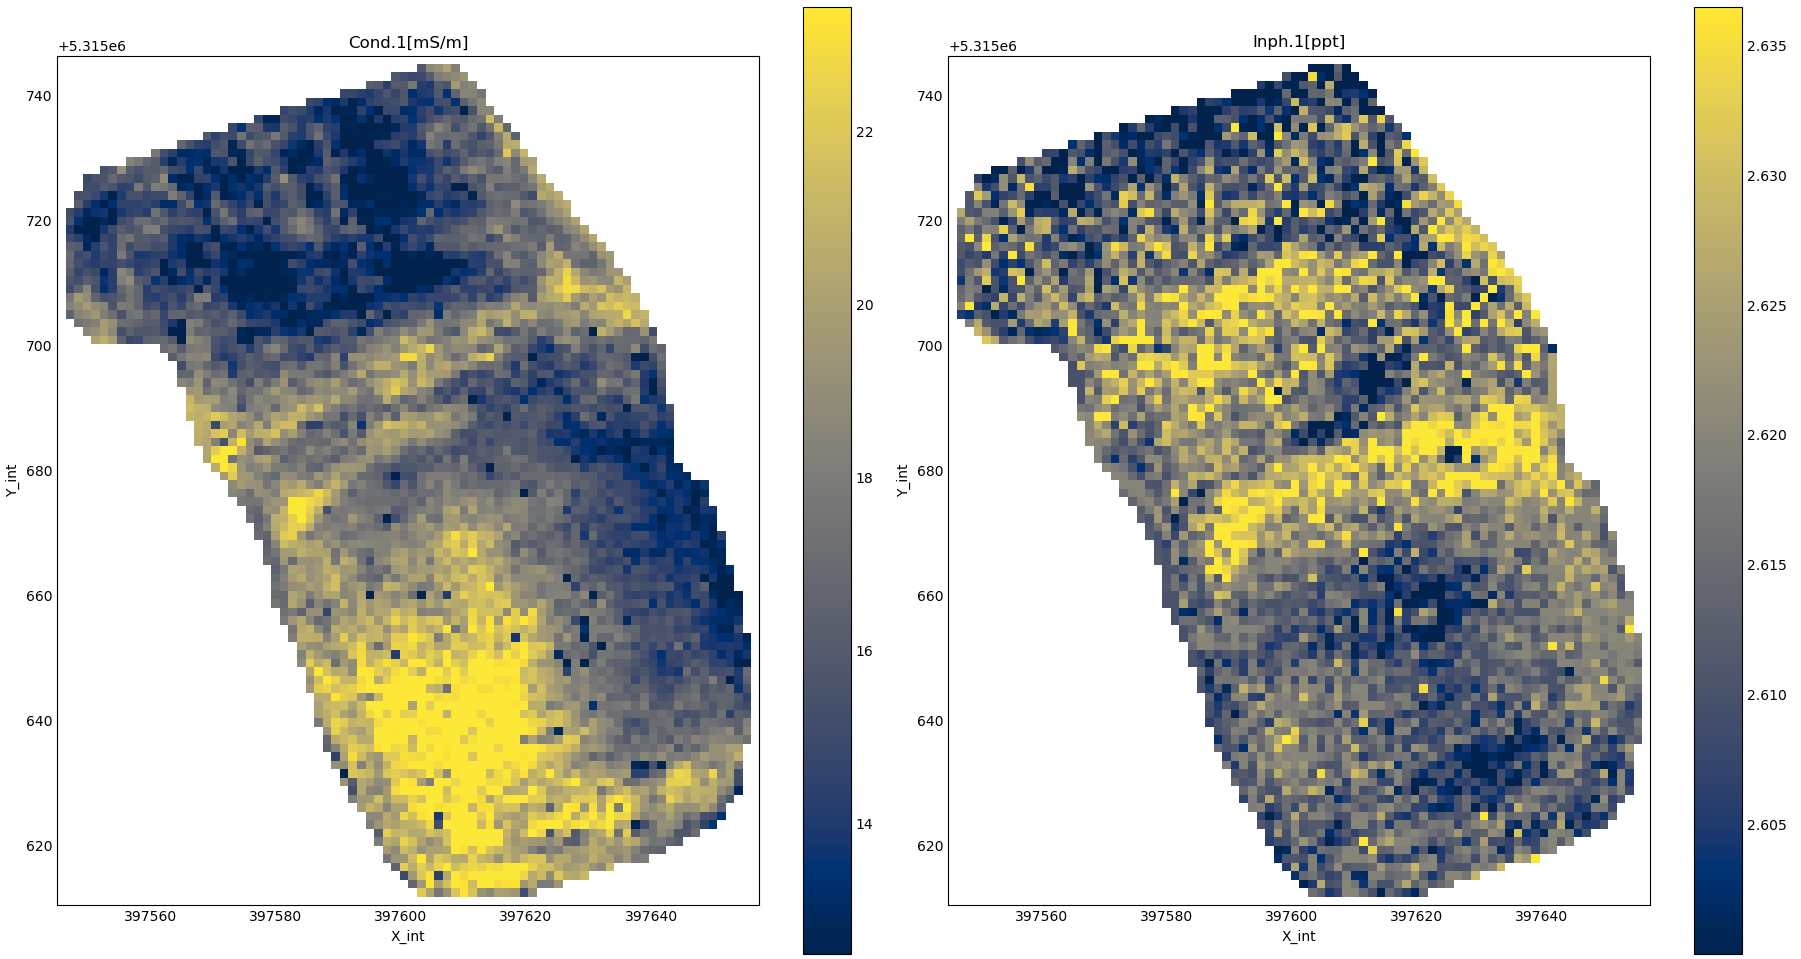
\includegraphics[width=0.8\textwidth]{Images/Grid_Interplin_r1c1p100.png}
        \caption{Interpolation linéaire, [\texttt{prec} = 100].}
    \end{figure}

    Il est important de noter que \texttt{scipy} possède automatiquement une option pour découper l'ensemble, mais elle ne le fait que de manière convexe. On crée donc de l'erreur.

    \begin{figure}[ht!]
        \centering
        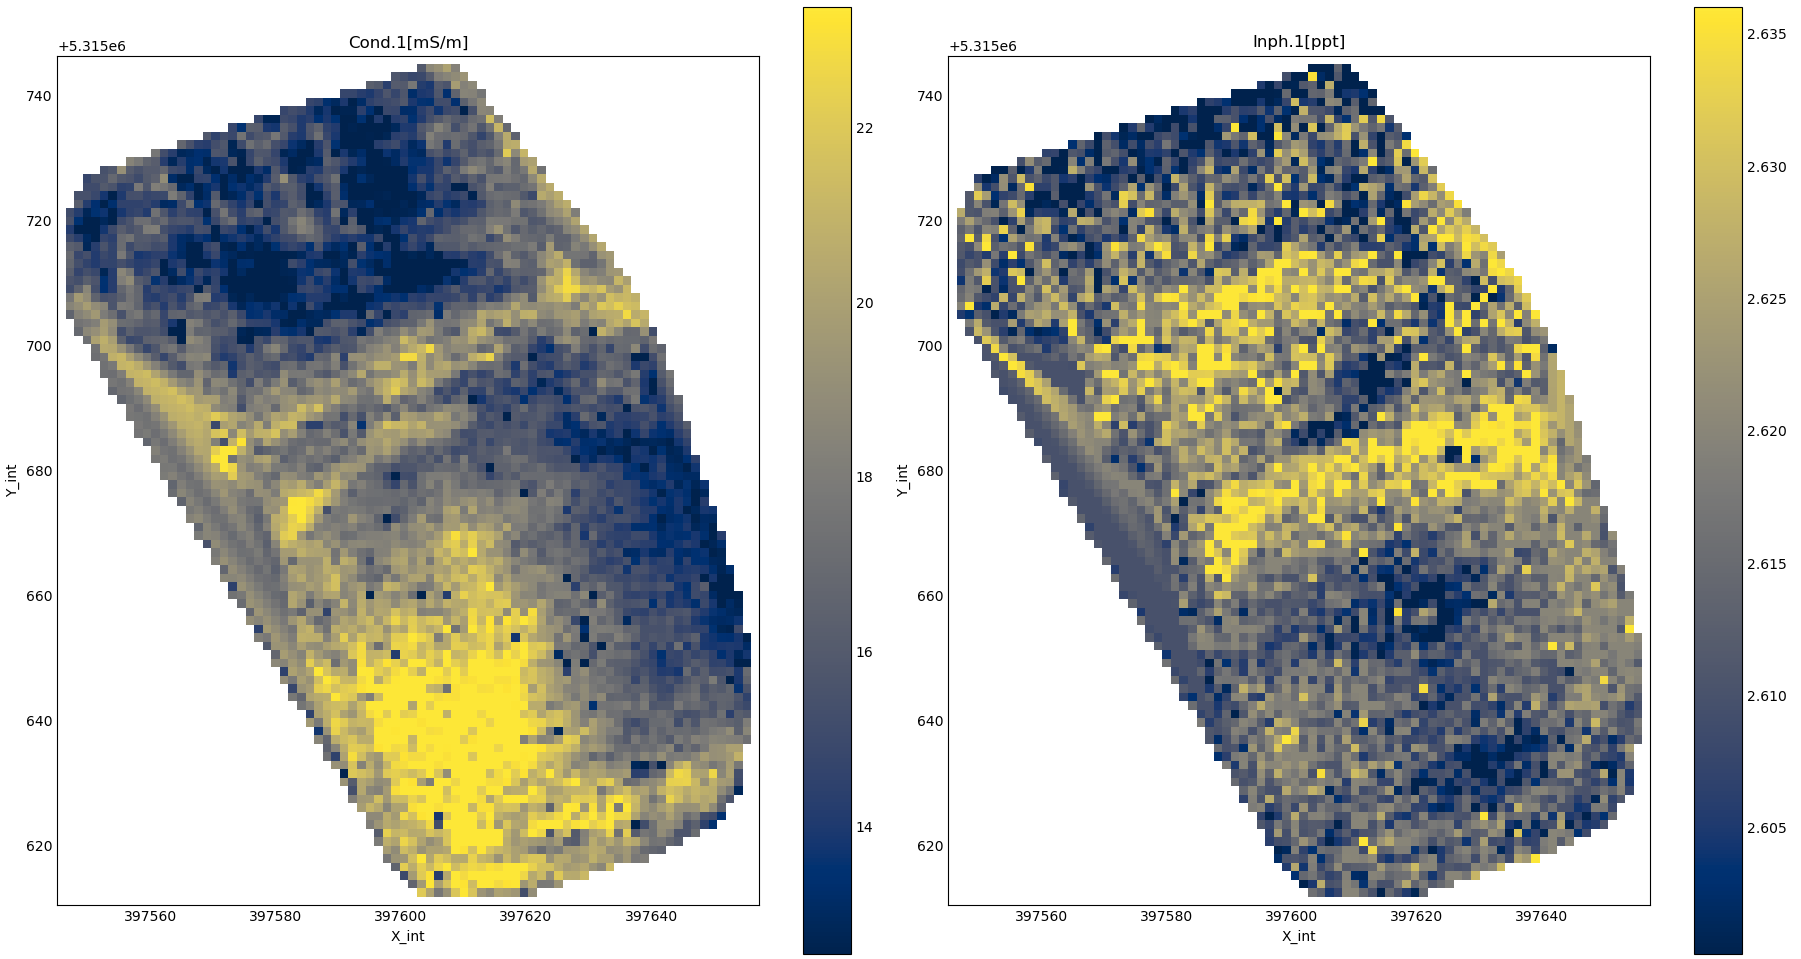
\includegraphics[width=0.8\textwidth]{Images/Grid_Interplin_r1c1p100_nocrop.png}
        \caption{Interpolation linéaire avec découpage convexe, [\texttt{prec} = 100].}
    \end{figure}

\subsubsection{Krigeage}

    Le \href{https://www.publichealth.columbia.edu/research/population-health-methods/kriging-interpolation#:~:text=Kriging%20is%20one%20of%20several,over%20a%20continuous%20spatial%20field.}{krigeage} est une méthode d'interpolation complexe cherchant à construire un variogramme (une loi d'évolution de la variance) qui colle le plus possible à celle mesurée sur le jeu de données.

    Il existe plusieurs librairies Python effectuant le krigeage, comme par exemple \href{https://gstlearn.org/}{gstlearn}.

    Cette partie ne sera pas détaillée car elle nécessite énormément de puissance de calcul (difficile de générer de belles figures), et la mise en place n'est pas compréhensible sous forme de résumé.

\subsubsection{Autres intérêts}

    Il existe des cas ou la visualisation classique (en nuage de points) ne soit pas adapté. Par exemple lors des prospections en carré on espace chaque profil d'un mètre, mais on prend un point tous les 20 centimètres. On a donc une densité verticale et horizontale bien différente, qui entraine des biais visuels en ligne (\ref{2_detec_front_ex2_in}). On se sert de l'interpolation pour harmoniser les variations.

    De même manière, on peut effacer les variations en oscillation récurrentes, qui sont dûes à l'appareil plutôt qu'au terrain (même jeu, \texttt{Cond.1[mS/m]}).

\newpage
\section{Interface shell/terminal}

    En complément des fonctions, j'ai développé un interface sur terminal (ou shell Python). Il sert à éviter de créer des scripts séparés en appelant directement les procédures. Les manipulations enregistrent donc automatiquement les résultats dans des fichiers de sortie. Cet interface pourra par la suite être utilisé par un interface graphique.
    
    L'utilisation du programme doit respecter les critères suivant :
    \begin{enumerate}
        \item[$\bullet$] \textbf{Accessible} : Le programme doit pouvoir être utilisé sans connaissances particulières en programmation. On s'attend cependant à ce l'utilisateur soit géophysicien ou au minimum conscient des notions scientifiques  s'y rattachant.
        \item[$\bullet$] \textbf{Rapide} : Rentrer les données nécessaires au traitement doivent prendre le moins de temps possible.
        \item[$\bullet$] \textbf{Modulable} : L'utilisateur doit pouvoir rentrer les paramètres des fonctions sans modifier le code.
        \item[$\bullet$] \textbf{Documenté} : Les fonctionnalités doivent être facilement accessibles, et leur utilisation claire. En particulier, on peut au minimum avoir accès au rôle de chaque fonction et à leurs paramètres requis.
        \item[$\bullet$] \textbf{Concis} : Il doit pouvoir fournir le maximum d'information utile à l'utilisateur, et le moins d'information superflues propres au code.
    \end{enumerate}

    Via le terminal, il est possible d'exécuter un script Python avec des paramètres. Il suffit de compléter la commande \texttt{python3 script.py} par une série chaine de caractères séparés par des espaces, comme par exemple \texttt{python3 script.py 9 argument "[0,1]"}. L'ordre de ces arguments est important. Les paramètres optionnels doivent être déclarés en dernier ; leur ordre peut être quelconque mais il faut préciser leur nom : \texttt{arg1=0}. La nomenclature tente de s'approcher le plus possible d'une fonction Python.

    En général, la format d'un appel se construit comme suit :
    
    \texttt{python3 Traitement\_CMD\_vX.py [nom\_fonction] [args\_principaux] [args\_optionnels]}.

    Si on souhaite simuler un appel de script depuis un shell IPython, on peut utiliser la commande \texttt{runfile} :
    
    \texttt{runfile('Traitement\_CMD\_vX.py',args='[nom\_fonction] [args\_ppaux] [args\_opts]')}

    De plus, il est toujours possible d'appeler les fonctions Python depuis le shell, ou alors d'utiliser les fonctions dans un script séparé. Dans ce cas, il vaut mieux se référer à la documentation interne au code (\textit{docstring}) pour avoir tous les bons arguments.
    
    Si aucun argument est spécifié lors de l'exécution, le programme propose de donner la documentation pour une fonction au choix, ou de toute les fonctions disponibles. Elle comprend un court résumé de son utilité, la liste des paramètres (obligatoires ou optionnels) ainsi que leur type et rôle, puis des exemples d'utilisation.

    \label{3_intter_out} En appelant la fonction d'aide \texttt{CMD\_help} et en spécifiant une fonction ou un numéro, seule celle sélectionnée sera affichée (\ref{3_intter_in}).

\newpage
\section{Interface graphique}

    En parallèle du terminal, il est possible d'utiliser un interface graphique simpliste pour ne pas taper les commandes à la main.

    \label{4_intgr_out} \label{4_intgr_k_out} Il comprend plusieurs menus (\ref{4_intgr_in}) répertoriant toutes les fonctions du terminal, groupées à par type (préfixes). Chaque écran de fonction (\ref{4_intgr_k_in}) comporte les éléments suivants :

    \begin{enumerate}
        \item[$\bullet$] Un espace pour rentrer la valeur de chaque variable. On précise le nom du paramètre, son type et sa valeur par défaut. Un paramètre requis est indiqué par une asterisque rouge.

        \item[$\bullet$] Un bouton exécutant la commande en ouvrant un terminal. Cette opération ne vérifie pas la validité des paramètres et laisse cette tâche au terminal.

        \item[$\bullet$] Si la fonction produit un résultat graphique, un bouton permet d'afficher la sortie stockée dans un dossier \texttt{Output}. Le dossier est vidé avant chaque exécution via fenêtre graphique. Par défaut, l'affichage produit les figures matplotlib (en fenêtres séparées) et les images. Il est ensuite possible de naviguer entre les images avec des boutons numérotés. À noter que l'affichage est indépendant de l'exécution, il est donc possible de prendre un résultat obtenu par d'autres moyens.

        \item[$\bullet$] Si la fonction produit un résultat graphique, un bouton permet de fermer les figures matplotlib. Puisque les figures ouvertes pendant l'exécution sont inactives, la croix ne marche pas.

        \item[$\bullet$] Le rôle de la fonction, tel qu'il est présenté dans l'aide.

        \item[$\bullet$] Un bouton pour afficher l'aide de la fonction dans un terminal. Un bouton pour quitter le menu. Un boutons pour afficher et modifier les options (voir ci-dessous).
    \end{enumerate}

    Changer la valeur de l'option pendant l'exécution n'impacte que l'exécution en cours. Si on veut modifier sa valeur définitivement, on pourra le faire via le fichier \texttt{CONFIG.py}.

%\newpage
\section{Librairie Python}
\subsection{Migration du code en module Python}

    Un des objectifs du stage est de reporter l'ensemble des procédures dans la librairie Python \texttt{geophpy}. Il s'agit d'une librairie créé et maintenue par un groupe informel dont font partie Éveha et Metis. Elle regroupe plusieurs procédures pour traiter des données géophysiques.

    Cependant, due à son ancienne date de création, elle n'utilise pas toutes les librairies usuelles comme \texttt{pandas}. De plus, son organisation interne doit être changée. Au vu de ma méconnaissance des fonctionalités déjà présentes, je n'ai fait qu'ajouter en l'état mes fonctions sans me soucier de copier la structure déjà existante.

    Pour lister les principaux changements dû au format :
    \begin{enumerate}
        \item[$\bullet$] Changements appliqués à l'ancien et au nouveau format :

        \begin{enumerate}
            \item[$\star$] Toutes les fonctions ou procédures reposant sur un interface dynamique (intervention utilisateur) doivent être automatisables. Pour cela, des paramètres spéciaux sont ajoutés auxquelles on peut préciser à l'avance les valeurs que l'interface demande.

            Pour l'interface de la frontière, la solution n'est que partiellement satisfaisante car l'ajustement fait intervenir une part d'aléatoire.

            \item[$\star$] Les fonctions sont commentées en français (privé).

            \item[$\star$] Les documentations (docstrings) sont rédigées en anglais (public).
        \end{enumerate}
        
        \item[$\bullet$] Changements uniquement appliqués au nouveau format :

        \begin{enumerate}
            \item[$\star$] Les messages d'erreurs customs sont remplacés par des erreurs Python (\texttt{raise}).

            \item[$\star$] Les nom des fonctions perdent leur préfixe.

            \item[$\star$] Les noms de variables en français sont migrées en anglais, en particulier les noms des colonnes des dataframes.

            \item[$\star$] Retrait des options liées à l'interface graphique ou à la sauvegarde des figures.
        \end{enumerate}
    \end{enumerate}

%\newpage
\subsection{Rédaction de notebooks}

    Afin de contextualiser et de mettre en évidence le fonctionnement des fonctions, plusieurs notebooks mettent en application des exemples. L'avantage de ce format est que les résultats sont sauvegardés, ce qui signifie qu'un utilisateur n'a pas besoin de l'exécuter pour observer les figures. De plus, cela permet d'insérer des cellules de texte autour du code.

    \begin{enumerate}
        \item[$\bullet$] Le premier notebook construit le déroulé entier du traitement en suivant un exemple simple. Cela permet d'exposer la manière la plus rapide de procéder, qui pourra être reprise telle quelle.

        \item[$\bullet$] Le second détaille certains ajustements dans des cas compliqués. En particulier, il explique certaines structures de code qui réduisent le nombre d'erreurs sur les procédures d'ajustement (frontières, manuelles) ainsi que certains algorithmes alternatifs (pseudo-profils par exemple).

        \item[$\bullet$] Le troisième présente plusieurs fonctionnalités plus petites appelées par les procédures principales. Il s'agit de fractionner le traitement afin d'avoir un plus grand contrôle sur le déroulé.
        
        \item[$\bullet$] Le quatrième propose d'utiliser certaines opérations sur fichiers de données bruts, dans le cas où des erreurs forcent à modifier certains champs en amont du traitement.

        \item[$\bullet$] Le cinquième expose les méthodes autour de la création et la gestion d'un dictionnaire d'appareil. Cet objet contient tous les champs pouvant être importants (écartements des bobines, configuration, antenne GPS...) et est requis par certaines procédures.
    \end{enumerate}

\section{Responsabilité sociale et environnementale}

    L'ensemble du travail disponible intégré à \texttt{geophpy} est sous licence \href{https://www.gnu.org/licenses/gpl-3.0.en.html}{\texttt{GNU GPL v3}}, qui est open-source. La production publique est donc à but non lucratif, mais son utilisation pour le commanditaire (Éveha) représente un gain d'efficacité.

    Ce stage m'a permis d'effectuer pour la première fois des réflexions sur la compatibilité des codes. Le premier concerne la façon de prospecter. En fonction des logiciels, des appareils ou des habitudes de chaque géophysicien, certains paradygmes donnés par mes tuteurs ne sont plus vrais (noms de colonnes inconnus, trajectoires aléatoires...). Certaines procédures du code ne marche donc plus. On ne peut ainsi jamais être compatible de manière absolue, on doit constament peser le pour et le contre entre la compatibilité locale (fichiers des membres du laboratoire), pour les principaux utilisateurs, et globale (formes les plus répandues) si l'information existe.

    \vskip 15pt

    Les réflexions écologiques s'arrêtent à la minimisation de la complexité, qui répond en parallèle à un besoin d'optimisation. Les algorithmes les plus lourds (ajustement par loi physique, krigeage) doivent être utilisés qu'en cas de besoin de grande précision, le reste du traitement faisant la grande partie du travail. De cette manière, on n'exige pas de matériel cher et énergivore.

    On peut également considérer les applications du travail en hydrologie (domaine d'activité de METIS) pour cartographier les profondeurs, ou pour les procédures générales l'adaptation avec d'autres types de prospections (électrique, magnétique, sismique...).

%\newpage
\section{Conclusion}
\subsection{État de la production}

    Les tâches réalisées au cours de ce stage sont :

    \begin{enumerate}
        \item[$\bullet$] L'ajustement des données selon différents critères (bases, frontières, interpolations, valeurs manquantes...)
        \item[$\bullet$] La multiplicité des méthodes de représentation des données finales (nuage classique, grille)
        \item[$\bullet$] L'automatisation des phases de traitement, lorsque c'est possible. La possibilité de laisser l'utilisateur prendre la main, si la procédure le nécessite.
        \item[$\bullet$] Le stockage de configurations via fichier JSON.
        \item[$\bullet$] L'interface utilisateur via terminal (cmd ou shell Python), puis graphique.
        \item[$\bullet$] La rédaction d'un rapport complet d'activité décrivant chaque procédure et fonctionnalité et des informations sur l'utilisation.
        \item[$\bullet$] La rédaction de documentations pour les fonctions.
        \item[$\bullet$] L'intégration à une librairie Python, mise en forme des fonctions réalisées au format "module".
        \item[$\bullet$] La création de notebooks (.ipynb) servant d'exemples d'utilisation de fonctions.
    \end{enumerate}

    
    L'ensemble de ce travail a été intégré à la documentation et à \texttt{geophpy}. Les changements à apporter devraient consister en de l'amélioration (plus grande compatibilité, optimisation) ou du debug potentiel. Parmi les aspects qu'il sera à gérer :

    \begin{enumerate}
        \item[$\bullet$] Vérifier la compatibilité Windows et Mac (concerne en particulier les procédures utilisant des commandes système).
        \item[$\bullet$] Faire le lien entre les anciens formats de données de \texttt{geophpy} et les dataframes \texttt{pandas} majoritairement utilisés par mes programmes.
        \item[$\bullet$] S'occuper de l'installation et de la publication de la librairie.
        \item[$\bullet$] Continuer l'ajout de contenu, en particulier pour les prospections en dehors de l'électromagn-étisme ou la gestion des cartes.
    \end{enumerate}

\subsection{Avis personnel}

    Contrairement aux stages précédents, j'ai pu participer à un projet de moyen-long terme, c'est-à-dire que je n'attendais pas en permanence qu'on me donne du travail par des tâches de quelques heures. Cela est bien plus enrichissant intellectuellement, en plus d'être en application avec les compétences de MAIN. Bien sûr, un stage d'un mois ne peut être bien plus qu'un stage de découverte, qui permet en général d'intégrer l'ambiance d'entreprise et de l'équipe.

    En revanche, le travail s'est fait de manière assez solitaire. Personne ne modifiait les mêmes codes que moi, je n'ai pas eu à m'adapter au rythme de travail de d'autres collègues (sauf à de très rares occasions). C'est bien sûr assez confortable, mais c'est un point d'expérience que je devrai acquérir autrement que par des projets scolaires. Les stages de 6 mois, faisant office de pré-embauche, pourront probablement compléter ce manque.

    Le domaine d'activité des laboratoires m'a intéressé, même si je ne verrais pas travailler dans de la physique plus tard. Dû à ma méconnaissance de la géophysique, j'ai souvent chercher à isoler les éléments importants d'un problème pour construire une solution informatique qui ne nécessite pas de compréhension totale de la théorie. Il s'agit d'un exercice enrichissant et, je pense, important dans le travail de programmeur. Avec le temps bien sûr, on finit par mieux saisir la portée de son travail.

    

\section{Annexe}
\subsection{Auto-évaluation de stage}

    Les pages suivantes présentent le compte-rendu de l'auto-évaluation remplie début juillet. Les points sont valables pour la fin de stage également, à l'exception de "Communiquer à l’écrit de façon professionnelle, structurée et synthétique" (mes tuteurs m'ont conseillé plusieurs éclaircissements sur la rédaction et le plan du rapport).
    \includepdf[landscape=true,pages=-]{auto_evaluation_57109.pdf}

\subsection{Compléments}

    Les annexes sont divisées par section. Il est possible de retourner à l'extrait lié à la ressource en cliquant sur le numéro en cyan.

    \label{1_sch_app_in} (\ref{1_sch_app_out}) Appareil de prospection

    \begin{figure}[ht!]
        \centering
        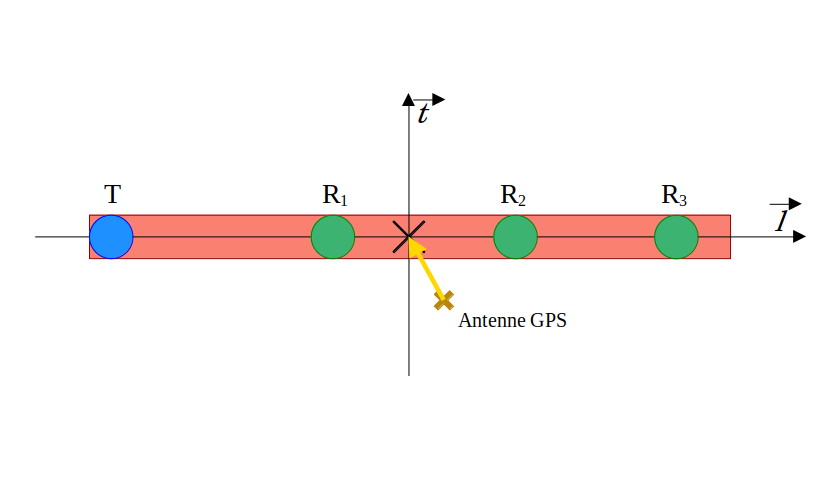
\includegraphics[width=\textwidth]{Images/SepVoies_Sch1.png}  
        \caption{Schéma simplifié de l'appareil de prospection électromagnétique, avec l'émetteur \texttt{T} et les récepteurs \texttt{R}.}
    \end{figure}

\newpage
    \label{2_detec_front_in} (\ref{2_detec_front_out}) Exemple de code (frontières)
    
\begin{lstlisting}
# Trouve un duo de points (l'un dans l'ensemble 1, l'autre dans le 2) le plus proche possible (excepté dans les sous-ensembles excl)

def CMD_appr_border(x1,x2,y1,y2,i_max,j_max,i_excl,j_excl):
    """ [TA]\n
    Find one point of each dataframe that are close to each other.\n
    They may not be included in the exclusion lists ``i_excl`` and ``j_excl`` to avoid duplicates.
    
    Notes
    -----
    This function does not provide the global minimum of distance, it converges to a fair enough pair.\n
    It runs through both lists and remove far points one by one (linear complexity).\n
    Starting points are taken randomly.
    
    Parameters
    ----------
    x1 : list of float
        X coordinates of first dataframe.
    x2 : list of float
        X coordinates of second dataframe.
    y1 : list of float
        Y coordinates of first dataframe.
    y2 : list of float
        Y coordinates of second dataframe.
    i_max : int
        Number of points of first dataframe.
    j_max : int
        Number of points of second dataframe.
    i_excl : list of int
        Exclusion list (indexes) of points of first dataframe.
    j_excl : list of int
        Exclusion list (indexes) of points of second dataframe.
    
    Returns
    -------
    i_min : int
        Selected point (index) of first dataframe.
    j_min : int
        Selected point (index) of second dataframe.
    d_min : float
        Distance between ``i_min`` and ``j_min``.
    
    See Also
    --------
    ``CMD_calc_frontiere``
    """
    i_dec = np.random.randint(0, i_max)
    j_dec = np.random.randint(0, j_max)
    while i_dec in i_excl:
        i_dec = np.random.randint(0, i_max)
    while j_dec in j_excl:
        j_dec = np.random.randint(0, j_max)
    i_min = i_dec
    j_min = j_dec
    i = 0
    j = 0
    i_ = i_dec - i_max
    j_ = j_dec - j_max
    d_min = (x1[i_min]-x2[j_min])**2 + (y1[i_min]-y2[j_min])**2
    turn = True
    
    # On parcourt les ensembles dans l'ordre de l'index à partir de points 
    # de départ aléatoires p1 et p2.
    # On parcourt le premier jeu jusqu'à trouver un point plus proche de p2 
    # que p1. Dans ce cas, il devient p1, et on itère sur l'autre jeu.
    # La démarche est identique avec p2.
    # On continue jusqu'à avoir exploré une fois tous les points des ensembles.
    # Complexité : O(n)
    while i < i_max or j < j_max:
        if turn:
            d = (x1[i_]-x2[j_min])**2 + (y1[i_]-y2[j_min])**2
            if d < d_min and i_%(i_max+1) not in i_excl:
                if j != j_max:
                    turn = False
                d_min = d
                i_min = i_%(i_max+1)
            elif i == i_max:
                turn = False
            else:
                i+=1
                i_+=1
        else:
            d = (x1[i_min]-x2[j_])**2 + (y1[i_min]-y2[j_])**2
            if d < d_min and j_%(j_max+1) not in j_excl:
                if i != i_max:
                    turn = True
                d_min = d
                j_min = j_%(j_max+1)
            elif j == j_max:
                turn = True
            else:
                j+=1
                j_+=1
    return i_min,j_min,d_min\end{lstlisting}

\newpage
    \label{2_detec_front_ex2_in} (\ref{2_detec_front_ex2_out}) Frontières avec choix manuel (exemple avec 5 parcelles carrées)

    \begin{figure}[ht!]
        \centering
        \begin{subfigure}[b]{\textwidth}
            \centering
            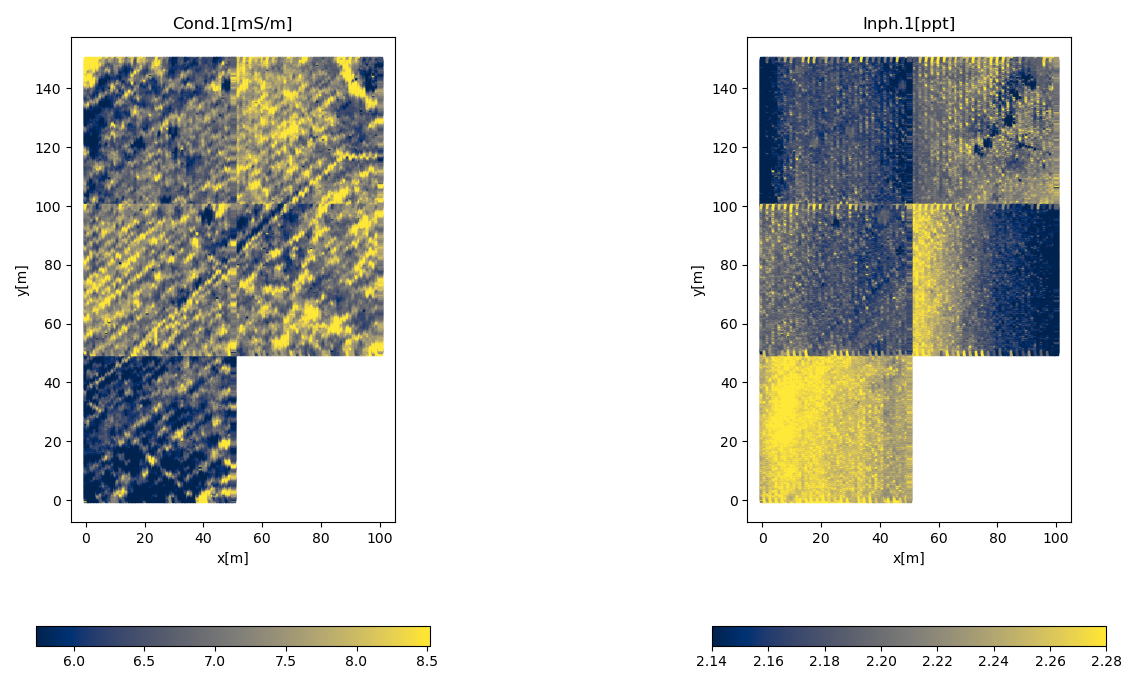
\includegraphics[width=0.85\textwidth]{Images/Frontiere_ex2_1.png}
            \caption[]%
            {{ \small Avant ajustement.}}    
        \end{subfigure}
        \centering
        \begin{subfigure}[b]{\textwidth}  
            \centering 
            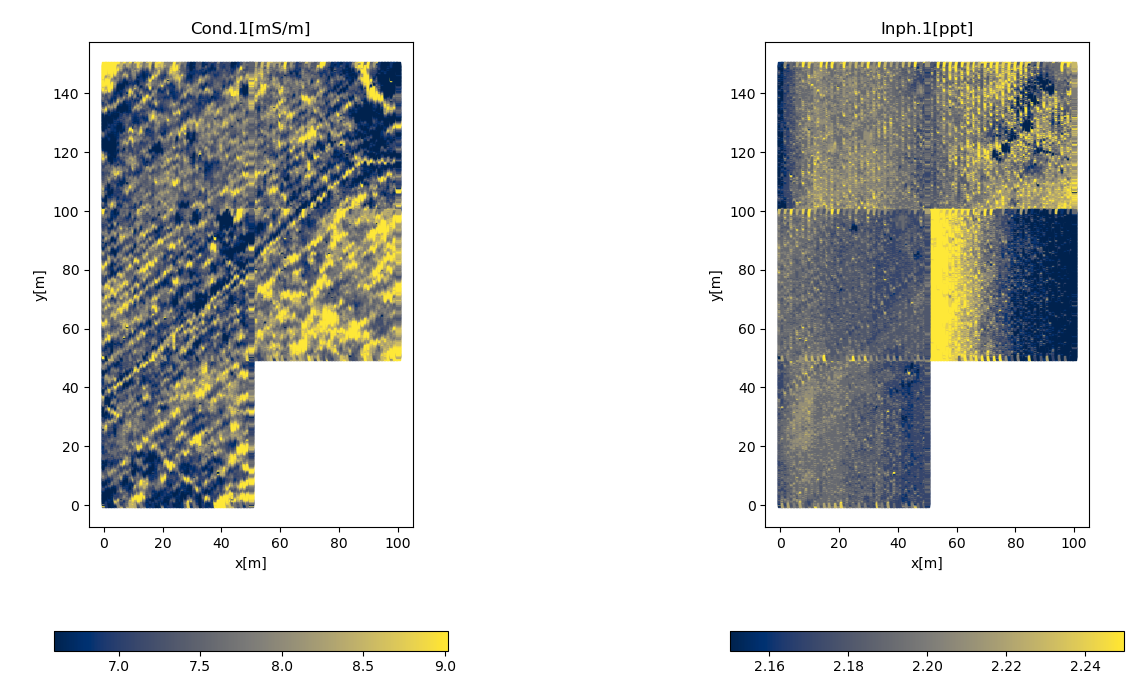
\includegraphics[width=0.85\textwidth]{Images/Frontiere_ex2_1_aj.png}
            \caption[]%
            {{\small Après ajustement.}}    
        \end{subfigure}
        \caption{Jeu 2018\_CMDm\_zone2, 1ère bobine.}
    \end{figure}
\newpage
    \begin{figure}[ht!]
        \centering
        \begin{subfigure}[b]{\textwidth}
            \centering
            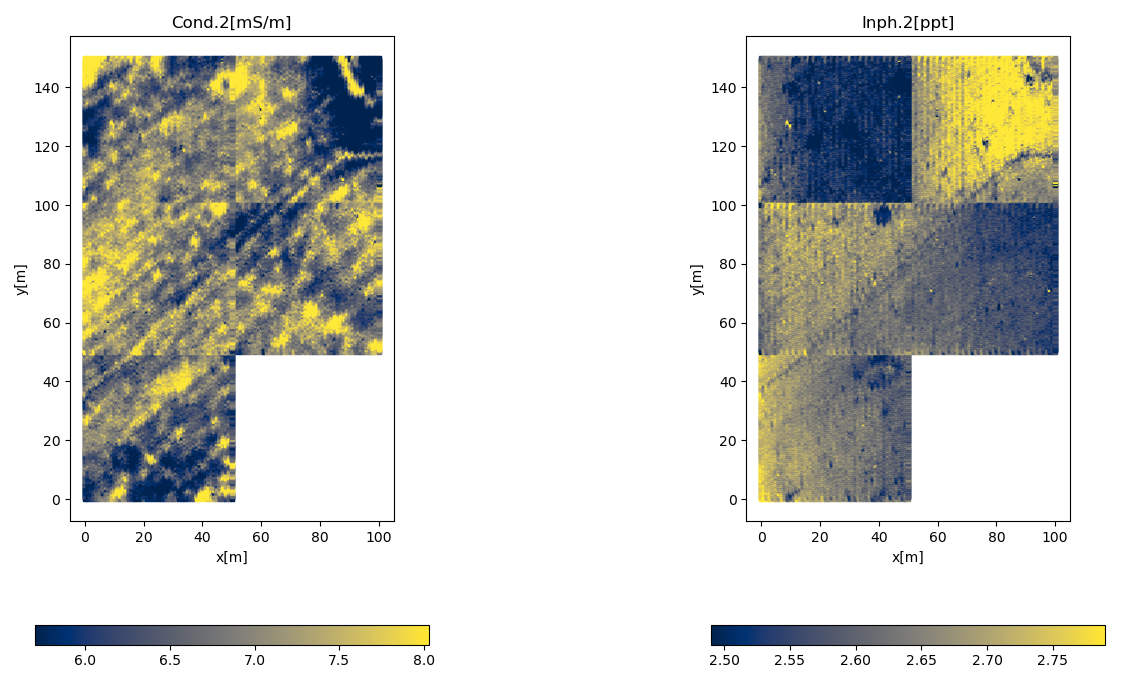
\includegraphics[width=0.9\textwidth]{Images/Frontiere_ex2_2.png}
            \caption[]%
            {{ \small Avant ajustement.}}    
        \end{subfigure}
        \centering
        \begin{subfigure}[b]{\textwidth}  
            \centering 
            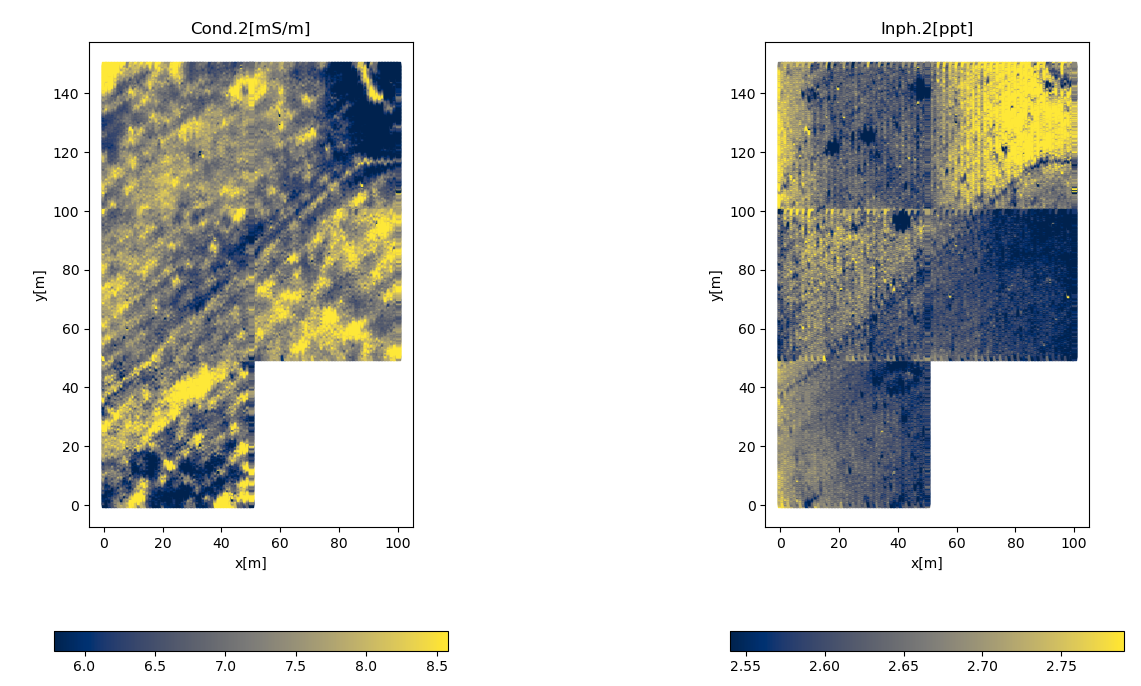
\includegraphics[width=0.9\textwidth]{Images/Frontiere_ex2_2_aj.png}
            \caption[]%
            {{\small Après ajustement.}}    
        \end{subfigure}
        \caption{Jeu 2018\_CMDm\_zone2, 2ème bobine.}
    \end{figure}
\newpage
    \begin{figure}[ht!]
        \centering
        \begin{subfigure}[b]{\textwidth}
            \centering
            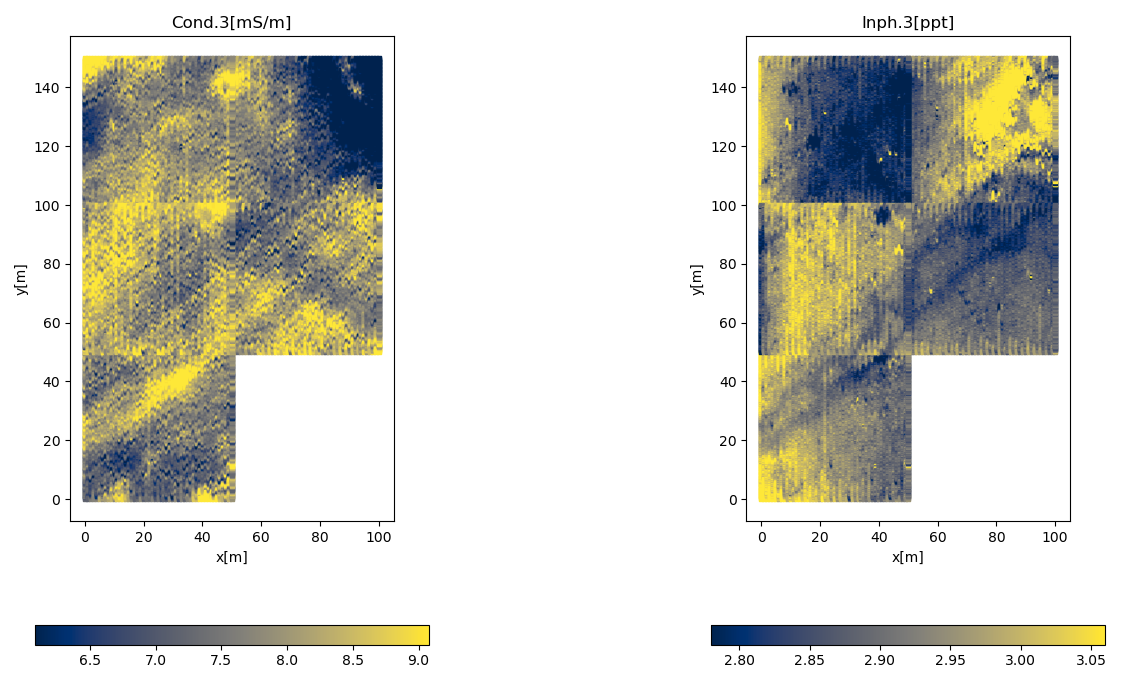
\includegraphics[width=0.9\textwidth]{Images/Frontiere_ex2_3.png}
            \caption[]%
            {{ \small Avant ajustement.}}    
        \end{subfigure}
        \centering
        \begin{subfigure}[b]{\textwidth}  
            \centering 
            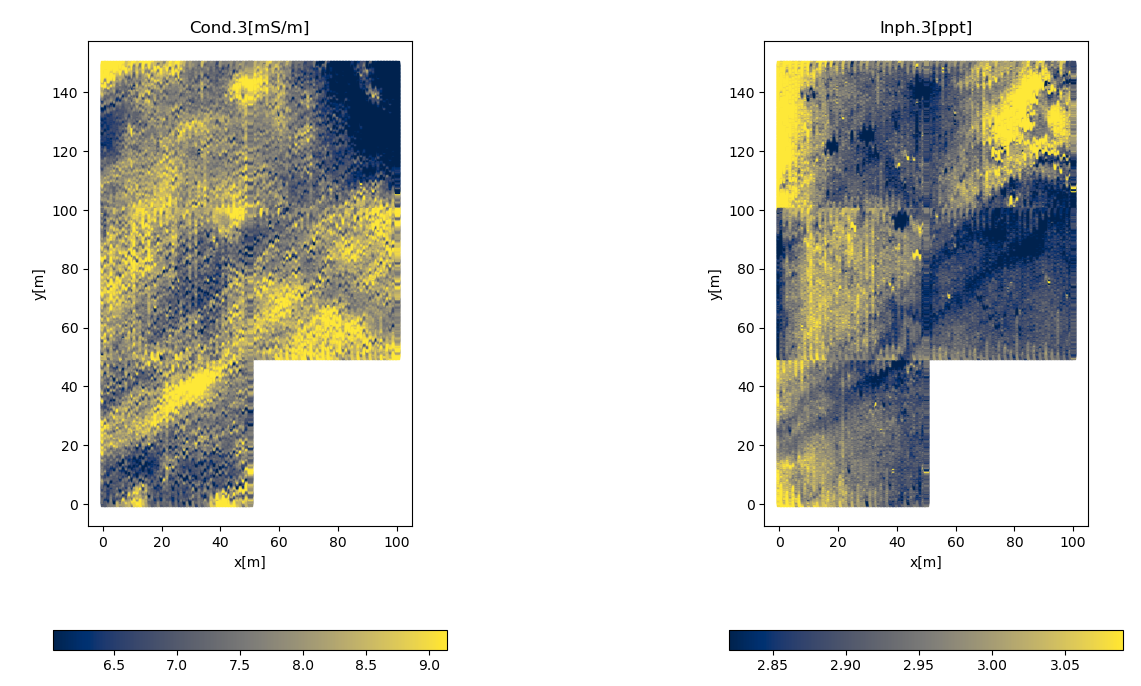
\includegraphics[width=0.9\textwidth]{Images/Frontiere_ex2_3_aj.png}
            \caption[]%
            {{\small Après ajustement.}}    
        \end{subfigure}
        \caption{Jeu 2018\_CMDm\_zone2, 3ème bobine.}
    \end{figure}

\newpage

    \label{2_aj_man_in} (\ref{2_aj_man_out}) Théorie de l'ajustement manuel

    \begin{figure}[ht!]
        \centering
        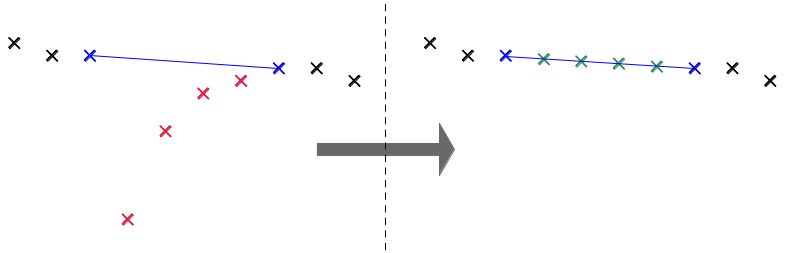
\includegraphics[width=\textwidth]{Images/Base_Schema_of_all_time.png}  
        \caption{Schéma représentatif de la procédure d'ajustement manuel.}
    \end{figure}

    \label{2_aj_man_ex_in} (\ref{2_aj_man_ex_out}) Exemple de l'ajustement manuel
    
    \begin{figure}[ht!]
        \begin{subfigure}[b]{0.475\textwidth}
            \centering
            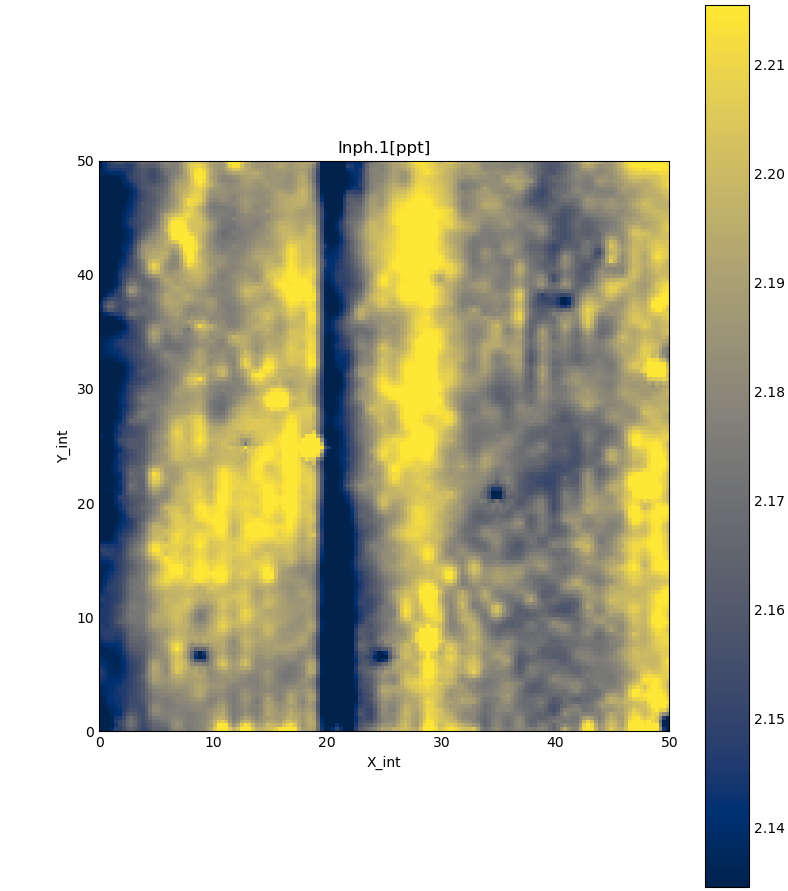
\includegraphics[width=\textwidth]{Images/Base_man_grid_Avant_sq1.png}
            \caption[]%
            {{ \small Affichage du jeu, avant ajustement.}}
        \end{subfigure}
        \hfill
        \begin{subfigure}[b]{0.475\textwidth}  
            \centering 
            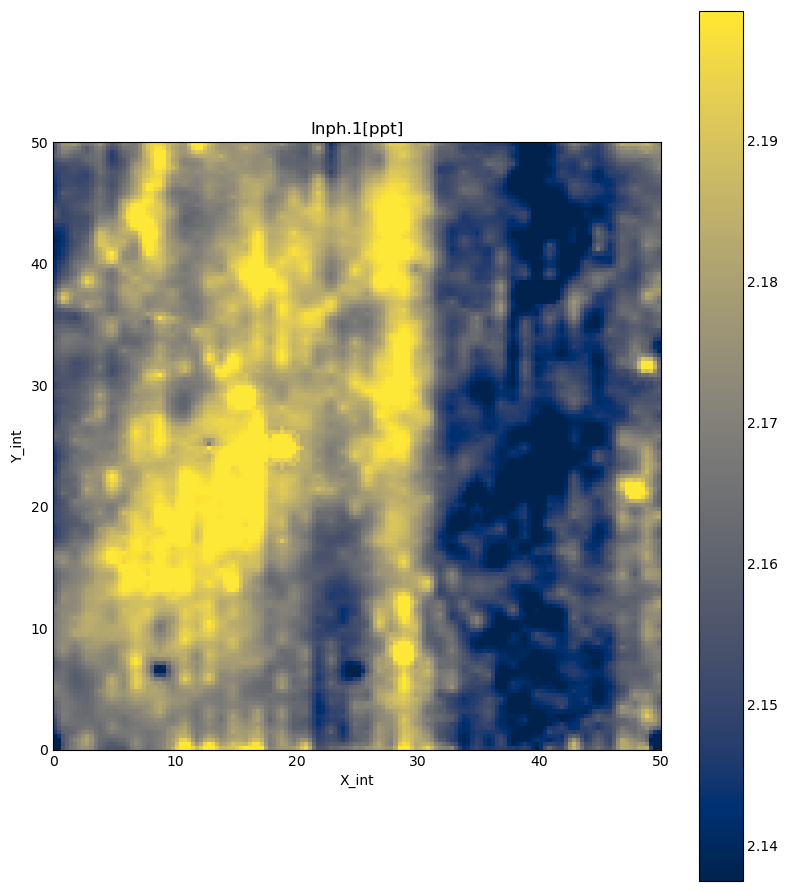
\includegraphics[width=\textwidth]{Images/Base_man_grid_Apres_sq1.png}
            \caption[]%
            {{\small Affichage du jeu, après ajustement.}}
        \end{subfigure}
        \caption{Ajustement sur deux bandes bleues (début et milieu).}
    \end{figure}

\newpage
    \label{2_grid_firstalg_coeff_in} (\ref{2_grid_firstalg_coeff_out}) Fenêtre de découpage

    \begin{figure}[ht!]
        \centering
        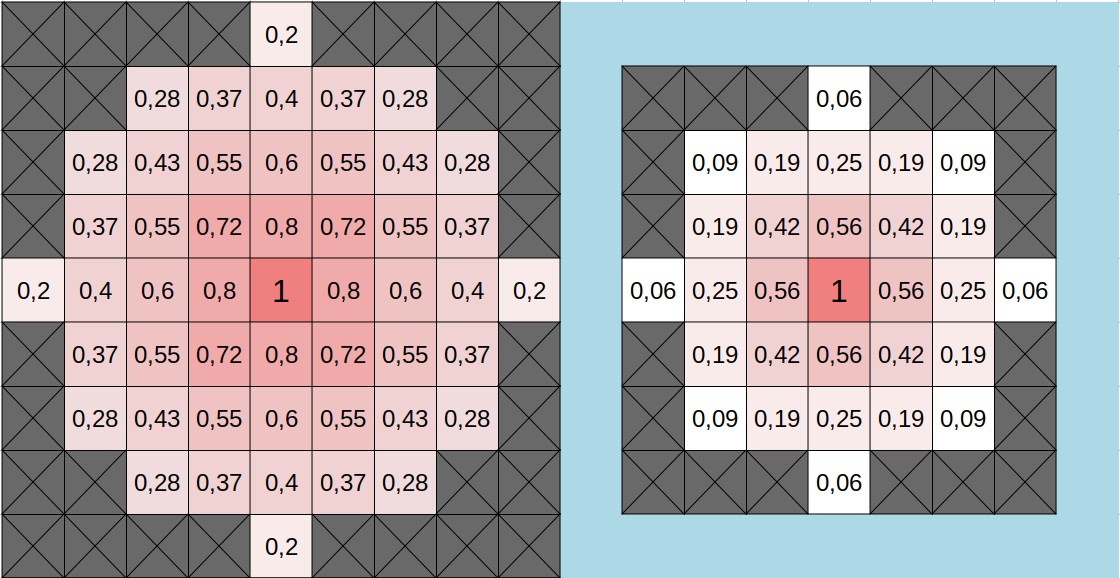
\includegraphics[width=\textwidth]{Images/Grid_FirstAlg_Coeff.png}  
        \caption{Grilles de coefficients, [$radius=4$,$seuil=1$] et [$radius=3$,$seuil=2$]}
    \end{figure}

    \label{3_intter_in} (\ref{3_intter_out}) Interface terminal (exemple d'aide)
    \begin{figure}[ht!]
        \centering
        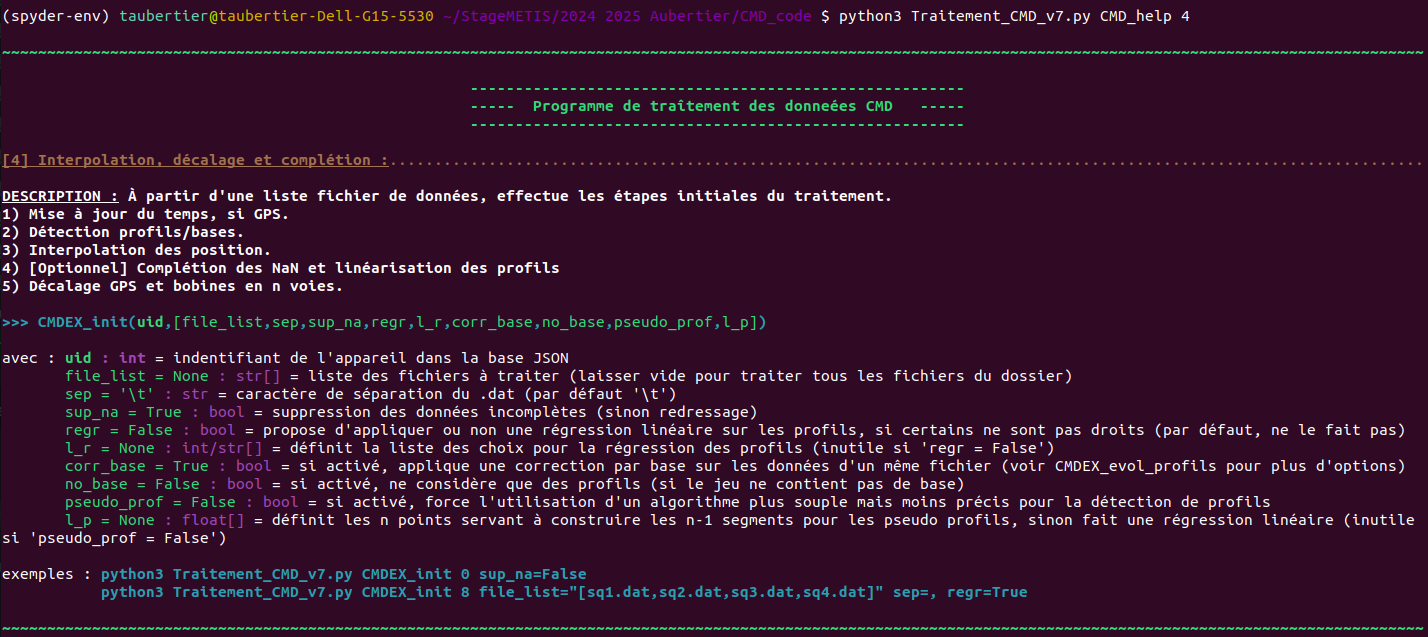
\includegraphics[width=\textwidth]{Images/IntTer.png}
        \caption{Description de fonction.}
    \end{figure}

\newpage
    \label{4_intgr_in} (\ref{4_intgr_out}) Interface graphique (menu principal)
    \begin{figure}[ht!]
        \centering
        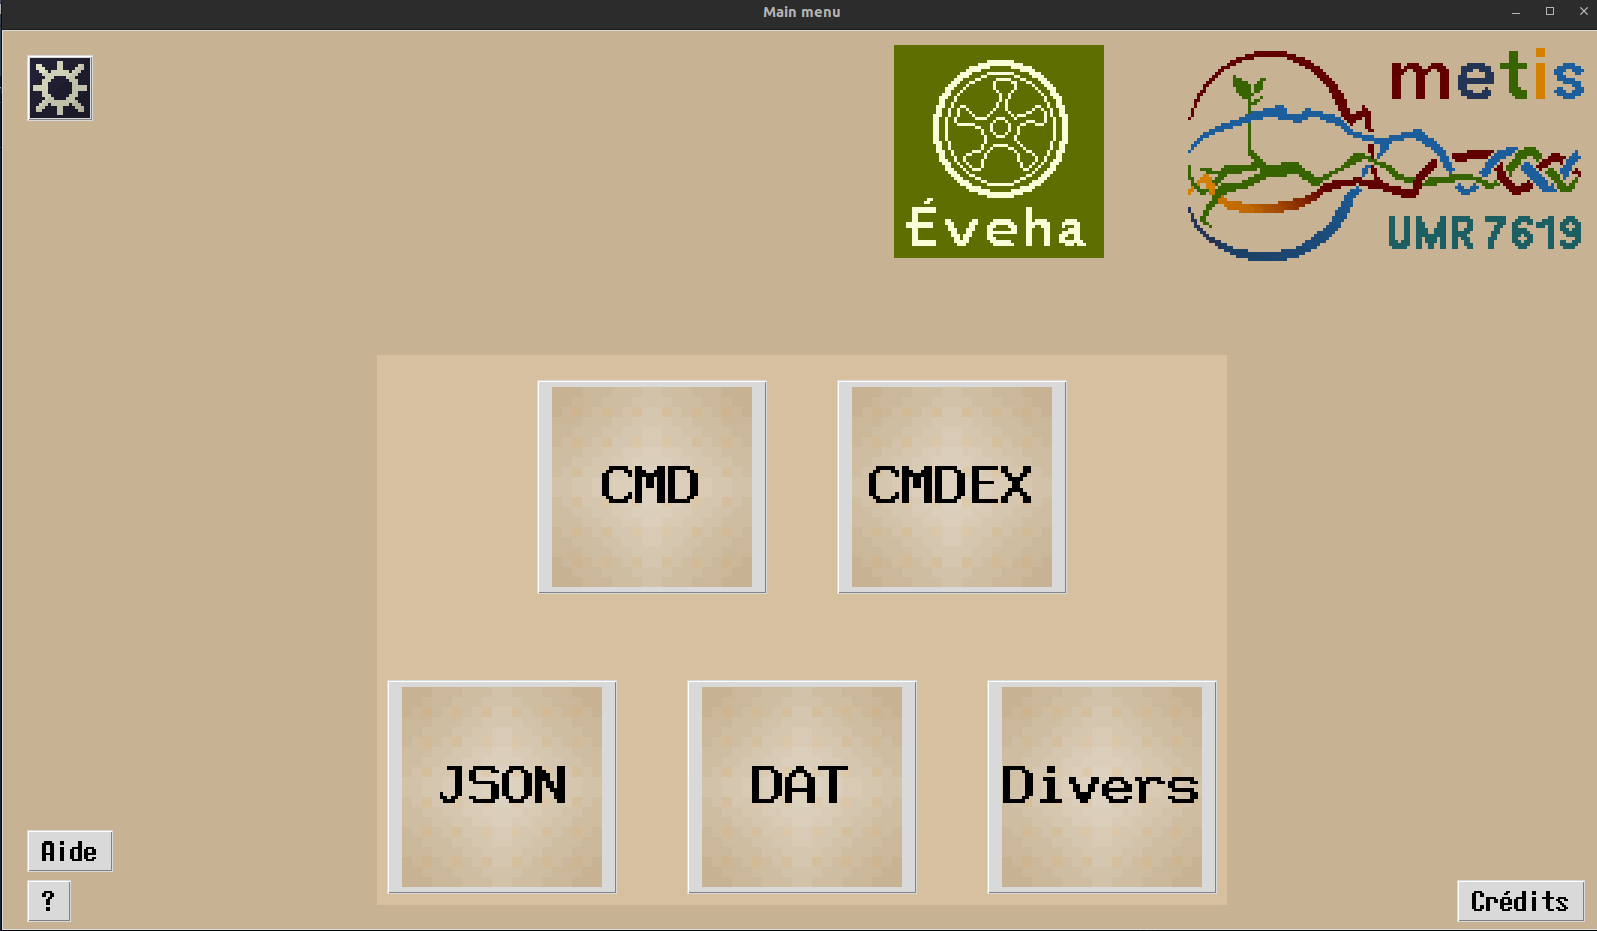
\includegraphics[width=0.9\textwidth]{Images/IntGraph_mm.png}
        \caption{Écran principal.}
    \end{figure}

    \label{4_intgr_k_in} (\ref{4_intgr_k_out}) Interface graphique (écran de fonction)
    \begin{figure}[ht!]
        \centering
        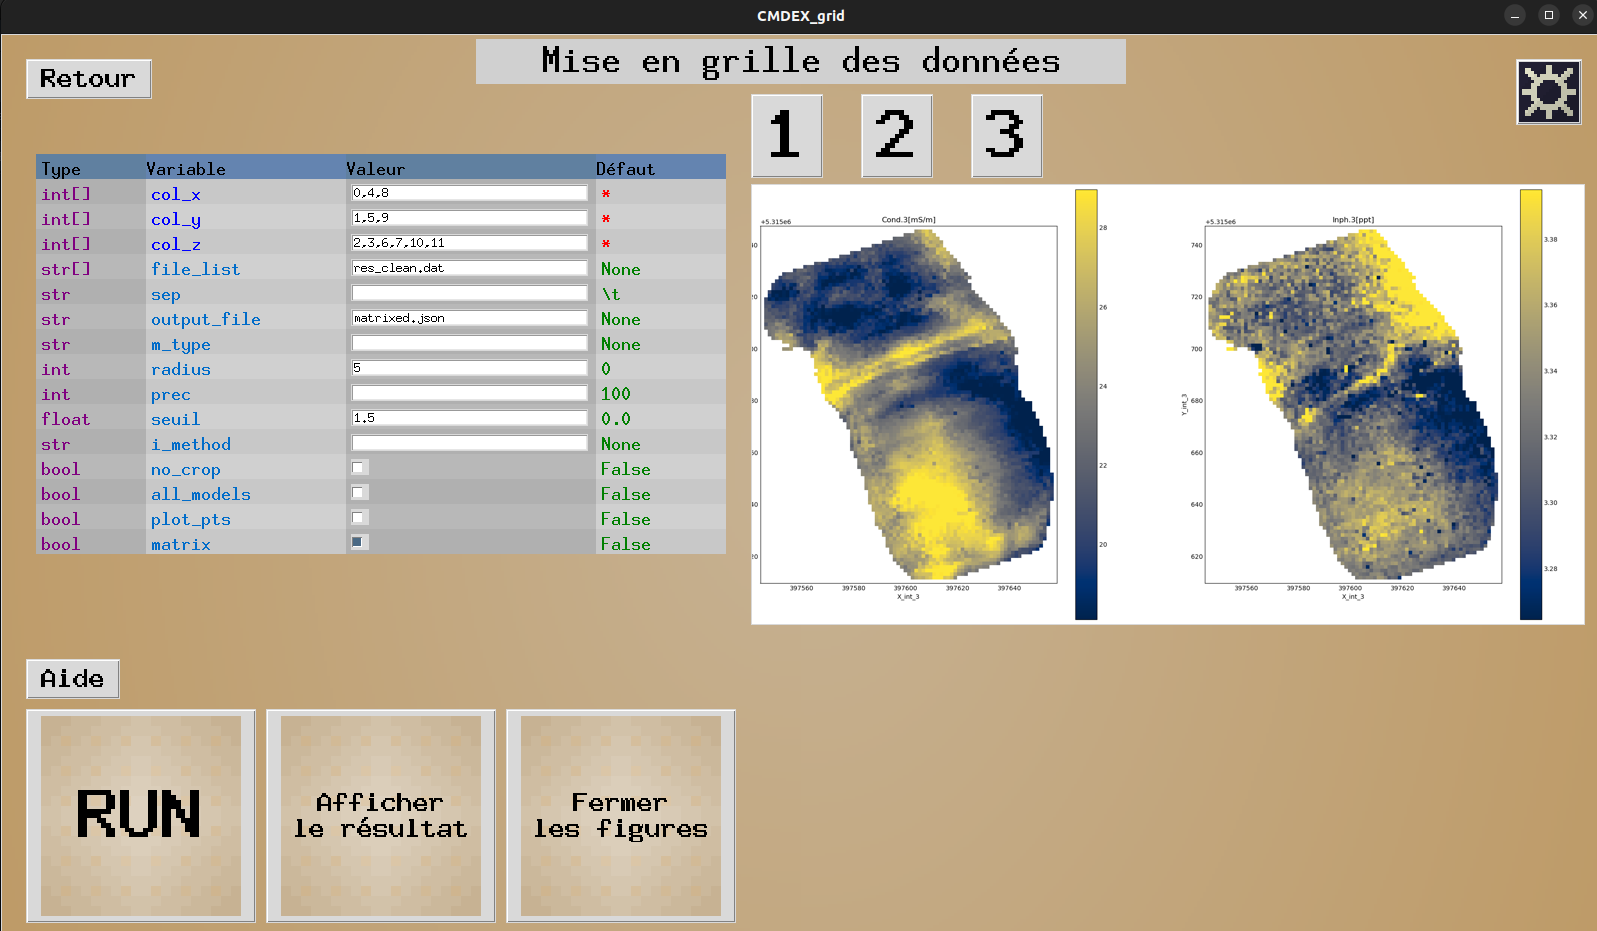
\includegraphics[width=0.9\textwidth]{Images/IntGraph_CMDEX_k.png}
        \caption{Exemple d'écran de fonction de traitement.}
    \end{figure}

\end{document}

